\documentclass[table, 12pt]{article}
\usepackage[T1]{fontenc}
\usepackage[utf8]{inputenc}
\usepackage[english]{babel}
\usepackage{graphicx}
\usepackage{titlesec}
\usepackage{hyperref}
\usepackage[usenames,dvipsnames]{xcolor}
\usepackage{float}
\usepackage[export]{adjustbox}
\usepackage{longtable}
\usepackage{mathtools}
\usepackage[most]{tcolorbox}
\newcounter{testexample}
\usepackage{xparse}
\usepackage{subcaption}
\usepackage{amsmath}

\hyphenation{Te-lan-ga-na}
\hyphenation{an-a-lys-ing}
\hyphenation{a-gron-o-mists}
\hyphenation{a-gron-o-mist}
\hyphenation{da-ta-base}
\hyphenation{ca-u-sed}
\hyphenation{Sen-sor-Da-ta-Ma-na-ger}
\hyphenation{Ac-count-Ma-na-ger}
\hyphenation{Lo-ca-tion-Mo-dule}
\titleformat{\paragraph}
{\normalfont\normalsize\bfseries}{\theparagraph}{1em}{}
\titlespacing*{\paragraph}
{0pt}{3.25ex plus 1ex minus .2ex}{1.5ex plus .2ex}


\def\exampletext{Example}

\NewDocumentEnvironment{testexample}{ O{} }
{
\colorlet{colexam}{teal!60!black} % Global example color
\newtcolorbox[use counter=testexample]{testexamplebox}{%
    % Example Frame Start
    empty,% Empty previously set parameters
    title={\exampletext #1},% use \thetcbcounter to access the testexample counter text
    % Attaching a box requires an overlay
    attach boxed title to top left,
       % Ensures proper line breaking in longer titles
       minipage boxed title,
    % (boxed title style requires an overlay)
    boxed title style={empty,size=minimal,toprule=0pt,top=4pt,left=3mm,overlay={}},
    coltitle=colexam,fonttitle=\bfseries,
    before=\par\medskip\noindent,parbox=false,boxsep=0pt,left=3mm,right=0mm,top=2pt,breakable,pad at break=0mm,
       before upper=\csname @totalleftmargin\endcsname0pt, % Use instead of parbox=true. This ensures parskip is inherited by box.
    % Handles box when it exists on one page only
    overlay unbroken={\draw[colexam,line width=.5pt] ([xshift=-0pt]title.north west) -- ([xshift=-0pt]frame.south west); },
    % Handles multipage box: first page
    overlay first={\draw[colexam,line width=.5pt] ([xshift=-0pt]title.north west) -- ([xshift=-0pt]frame.south west); },
    % Handles multipage box: middle page
    overlay middle={\draw[colexam,line width=.5pt] ([xshift=-0pt]frame.north west) -- ([xshift=-0pt]frame.south west); },
    % Handles multipage box: last page
    overlay last={\draw[colexam,line width=.5pt] ([xshift=-0pt]frame.north west) -- ([xshift=-0pt]frame.south west); },%
    }
\begin{testexamplebox}}
{\end{testexamplebox}\endlist}


\begin{document}
\begin{titlepage}
    \centering
    {\scshape\large AY 2021/2022 \par}
    \vfill
    
\includegraphics[width=100pt]{assets/logo-polimi-new}\par\vspace{1cm}
    {\scshape\LARGE Politecnico di Milano \par}
    \vspace{1.5cm}
    {\huge\bfseries DD\@: Design Document \par}
    \vspace{2cm}
    {\Large {Ottavia Belotti\quad Alessio Braccini\quad Riccardo Izzo}\par}
    \vfill
    {\large Professor\par
        Elisabetta \textsc{Di Nitto}}
    \vfill
    {\large \textbf{Version 1.0}\\ \today \par}
\end{titlepage}

\hypersetup{%
    pdfborder = {0 0 0}
}

\thispagestyle{plain}
\pagenumbering{gobble}
\mbox{}
\newpage
\pagenumbering{roman}
\tableofcontents
\newpage
\pagenumbering{arabic}

\section{Introduction}


\subsection{Purpose}
The purpose of this document is to provide a full technical description of the system described in the RASD document.
In this design document we discuss about both hardware and software architectures in terms of interaction among the components that represent the system.
Moreover, there are mentions about the implementation, testing and integration process.
This document will include technical language so it is primarily addressed to programmers, but stakeholders are also invited to read it in order to understand the characteristics of the development.

\subsection{Scope}
The scope of this design document lays in the definition of the system behavior, in both general and critical cases, and in the design of the system architecture by describing the
logical allocation of the components and the interaction between them.
This document also extends in part to the implementation and testing plan, where one possible course of action is explained, user interface design of user applications and requirements traceability relating to the RASD.
\subsection{Definitions, acronyms, abbreviations}
\subsubsection*{Definitions}
\begin{itemize}
    \item \textbf{Production entry}: the pair sown quantity and harvested quantity of a certain crop that the farmer inserts as his/her production.
    \item \textbf{Full production entry}: a production entry that carries both sown quantity and harvested quantity, even if inserted in different times of the year, as it normally should, since it is expected that the farmer will insert the sown quantity of crop during the sowing season and the harvested quantity during harvest. Every basic production entry should become a valid production entry.
\end{itemize}
\subsubsection*{Acronyms}
\begin{itemize}
    \item \textbf{DREAM}: \emph{Data-driven predictive farming}
    \item \textbf{RASD}: Requirement Analysis and Specification Document
    \item \textbf{DD}: Design Document
    \item \textbf{API}: Application Programming Interface
    \item \textbf{DBMS}: Database Management System
    \item \textbf{UML}: Unified Modeling Language
    \item \textbf{GPS}: Global Positioning System
    \item \textbf{IT}: Information Technology
    \item \textbf{GUI}: Graphic User Interface
    \item \textbf{UI}: User Interface
    \item \textbf{HTTPS}:HyperText Transfer Protocol Security
    \item \textbf{HTML}: HyperText Markup Language
    \item \textbf{CSS}: Cascade Style Sheet
    \item \textbf{JS}: JavaScript
\end{itemize}
\subsection{Revision history}
\begin{itemize}
    \item Version 1.0: initial version
    \item Version 1.1: update after the implementation
    \begin{itemize}
        \item[--] Update high-level-architecture: GoogleMaps and OpenWeather now communicates with the Web Server
        \item[--] Update component diagrams: LocationModule, MapServiceManager and WeatherManager now are in the Web Server, this changes are reflected also in the component interfaces diagram
        \item[--] Update deployment diagram: change hosting platform and load balancer
        \item[--] Delete EditProfile sequence diagram, update SignUp and CheckWeatherForecast sequence diagrams
        \item[--] Update integration and testing 
    \end{itemize}
\end{itemize}
\subsection{Reference documents}
\begin{itemize}
    \item Specification document: "Assignment RDD AY 2021-2022"
    \item Requirements Analysis Specification Document (RASD)
    \item UML documentation: https://www.uml-diagrams.org/
    \item ArchiMate documentation: https://pubs.opengroup.org/architecture/archimate3-doc/
    \item Slides of the lectures
\end{itemize}
\subsection{Document structure}
\begin{itemize}
    \item \textbf{Section 1} gives a brief description of the design document, it describes the purpose and the scope of it including all the definitions, acronyms and abbreviations used. 
    \item \textbf{Section 2} delves deeply into the system architecture by providing a detailed description of the components, the interfaces and all the technical choices made for the development of the application.
    It also includes detailed sequence, component and ArchiMate diagrams that describe the system in depth.
    \item \textbf{Section 3} contains a complete description of the user interface (UI), it includes all the client-side mockups with some graphs useful to understand the correct execution flow.
    \item \textbf{Section 4} maps the goals and the requirements described in the RASD to the actual functionalities presented in this DD.
    \item \textbf{Section 5} presents a description of the implementation, testing and integration phases of the system components that are going to be carried out during the technical development of the application.
\end{itemize}

\newpage
\section{Architectural Design}

\subsection{Overview}
\begin{center}
    \begin{figure}[H]
        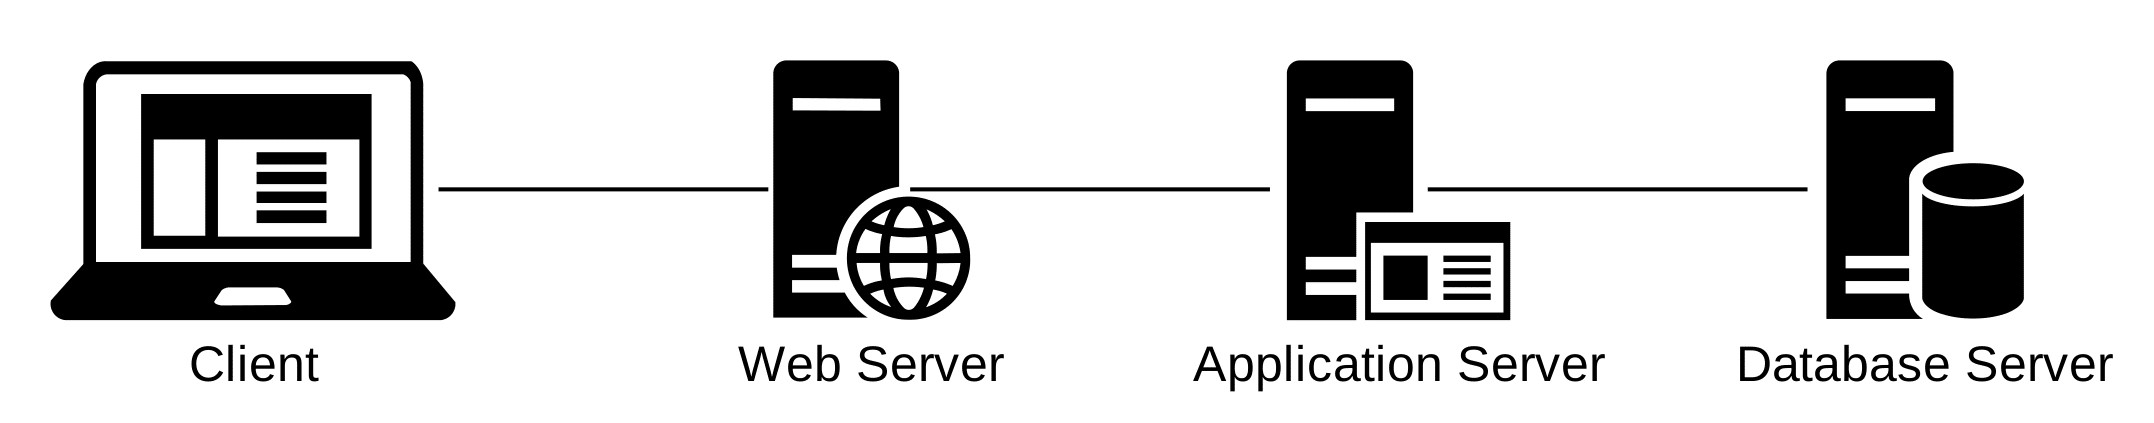
\includegraphics[scale=0.55, center]{assets/4-tier-scheme.jpg}
        \caption{Four-Tier Architecture Scheme}
        \label{fig: four-tier-architecture-scheme}
    \end{figure}
\end{center}

The system is a distributed application that follows the common client-server paradigm.
The architecture of the application is structured in three logic layers:
\begin{itemize}
    \item \textbf{Presentation Layer (P)}: it manages the presentation logic and handles the user actions.
    It is characterized by a GUI (Graphic User Interface) that allows the user to interact with the application in a simple and effective way.
    \item \textbf{Logic or Application Layer (A)}: it manages all the functionalities that has to be provided to the users, it is also responsible of data exchange between the client and the data sources.
    \item \textbf{Data Layer (D)}: it manages the access to data sources, it gets data from the database and moves it through the other layers.
    It is essential to guarantee a high level of abstraction from the database in order to provide an easy to use model.
\end{itemize}

\begin{center}
    \begin{figure}[H]
        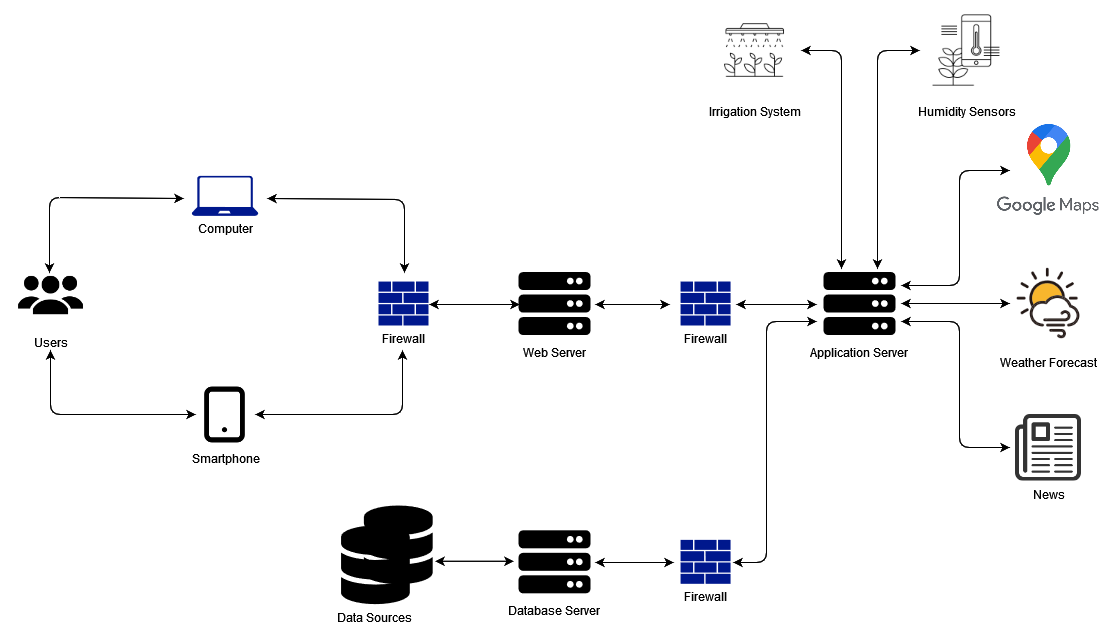
\includegraphics[scale=0.70, center]{assets/4-tier-architecture-scheme.png}
        \caption{High Level Architecture}
        \label{fig: high_level_architecture}
    \end{figure}
\end{center}

The system, as shown in \textit{Figure (\ref{fig: four-tier-architecture-scheme})}, is based on a four-tier architecture (Client, Web Server, Application Server and Database Server), this ensures more flexibility and high scalability.
The tiers are separated by firewalls in order to guarantee a higher level of security to the whole system.
A thin client is used to prevent heavy computation loads client side, in this way all the heavy operations are executed at server side.
The client's devices can be a personal computer, a mobile device or any kind of IT device able to connect to the Web Server through a web browser. In fact, the four-tiers architecture has been specifically chosen to allow the widest variety of commercial devices to access the application, without the need of developing an OS-specific one for each of them.
The Web Server manages the HTTP requests by the users and forwards them to the Application Server.
It also manages all the external APIs including GoogleMapsAPI and OpenWeatherAPI.
The first one enable the geolocalization while the other one allows to retrieve data like weather information directly from it in order to show them to the user.
The Application Server communicates with the Database Server and manipulates data following its business logic.
It also manages the external services such as the news, the water irrigation service and the humidity service.
Finally the Database Server manages all the internal data sources and communicates directly with the Application Server.
All the components will be described in depth in the following sections

\subsection{Component view}
\subsubsection*{General Component View}
\begin{center}
    \begin{figure}[H]
        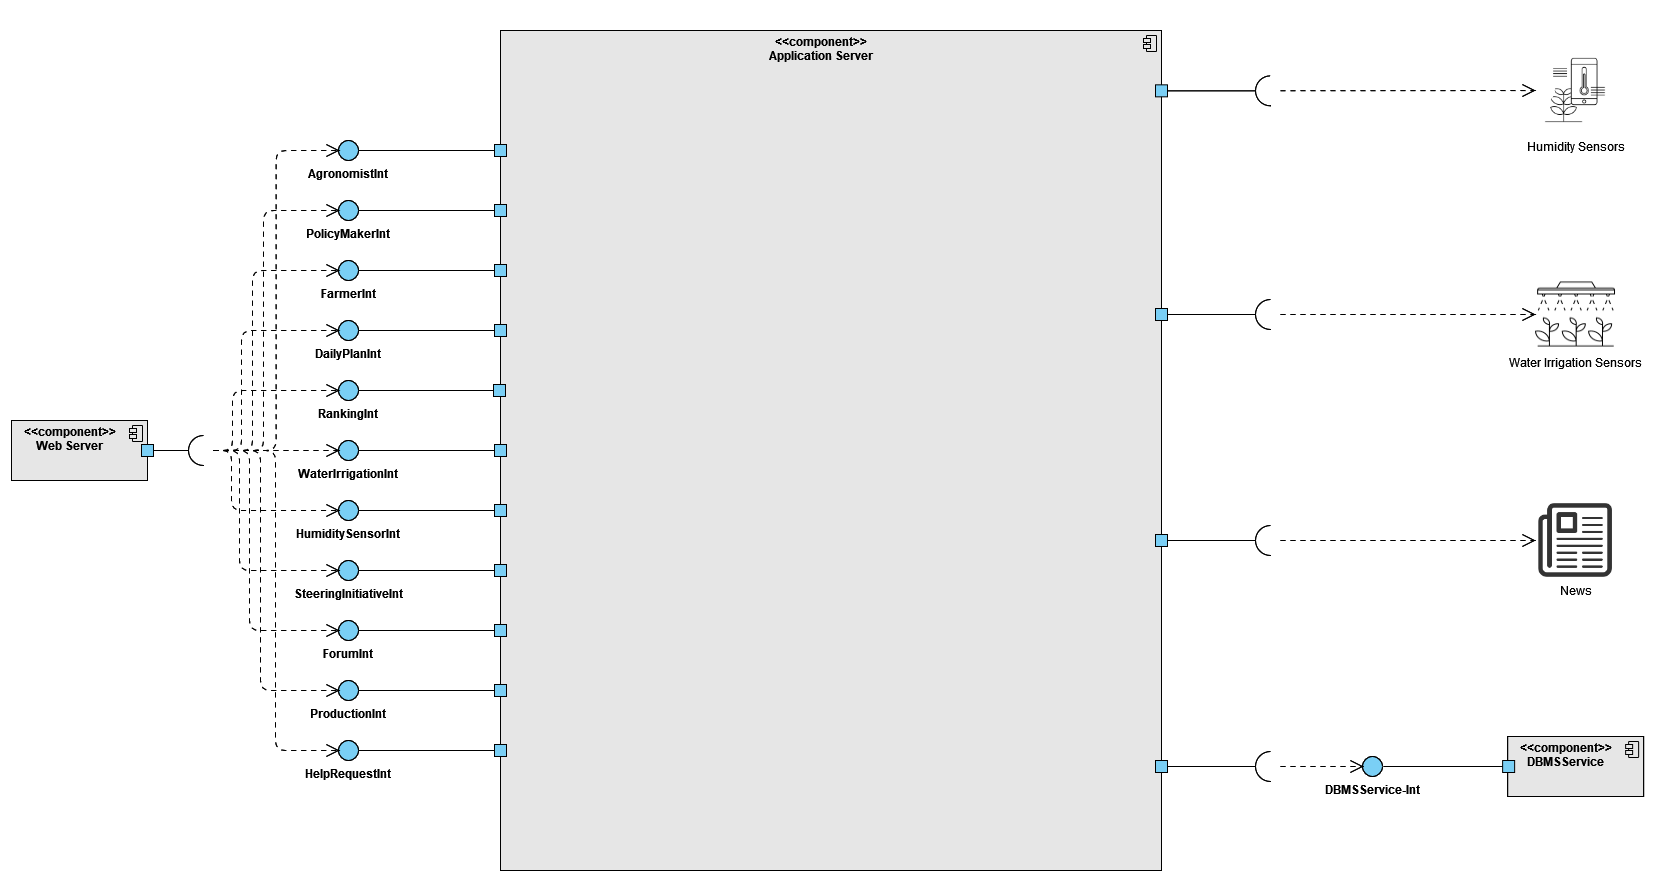
\includegraphics[scale=0.45, center]{assets/general-component-view.png}
        \caption{General Component Diagram}
        \label{fig: general_component_view}
    \end{figure}
\end{center}

This image gives a high level representation of the components of the system.
On the left are shown the provided interfaces between the Web Server and the Application Server that in this scheme is represented as a "black box", a complete description of it is provided in the next section.
All the interfaces basically represent the main functionalities requested by the client application.
On the right-hand side, there are the external requested interfaces. Among these there are the news, the water irrigation system and the humidity system.
Finally, the DBMS interface manages the DBMS service and it's responsible of the communication between the Application Server and the Database Server.

\subsubsection*{Application Server Component View}
\begin{center}
    \begin{figure}[H]
        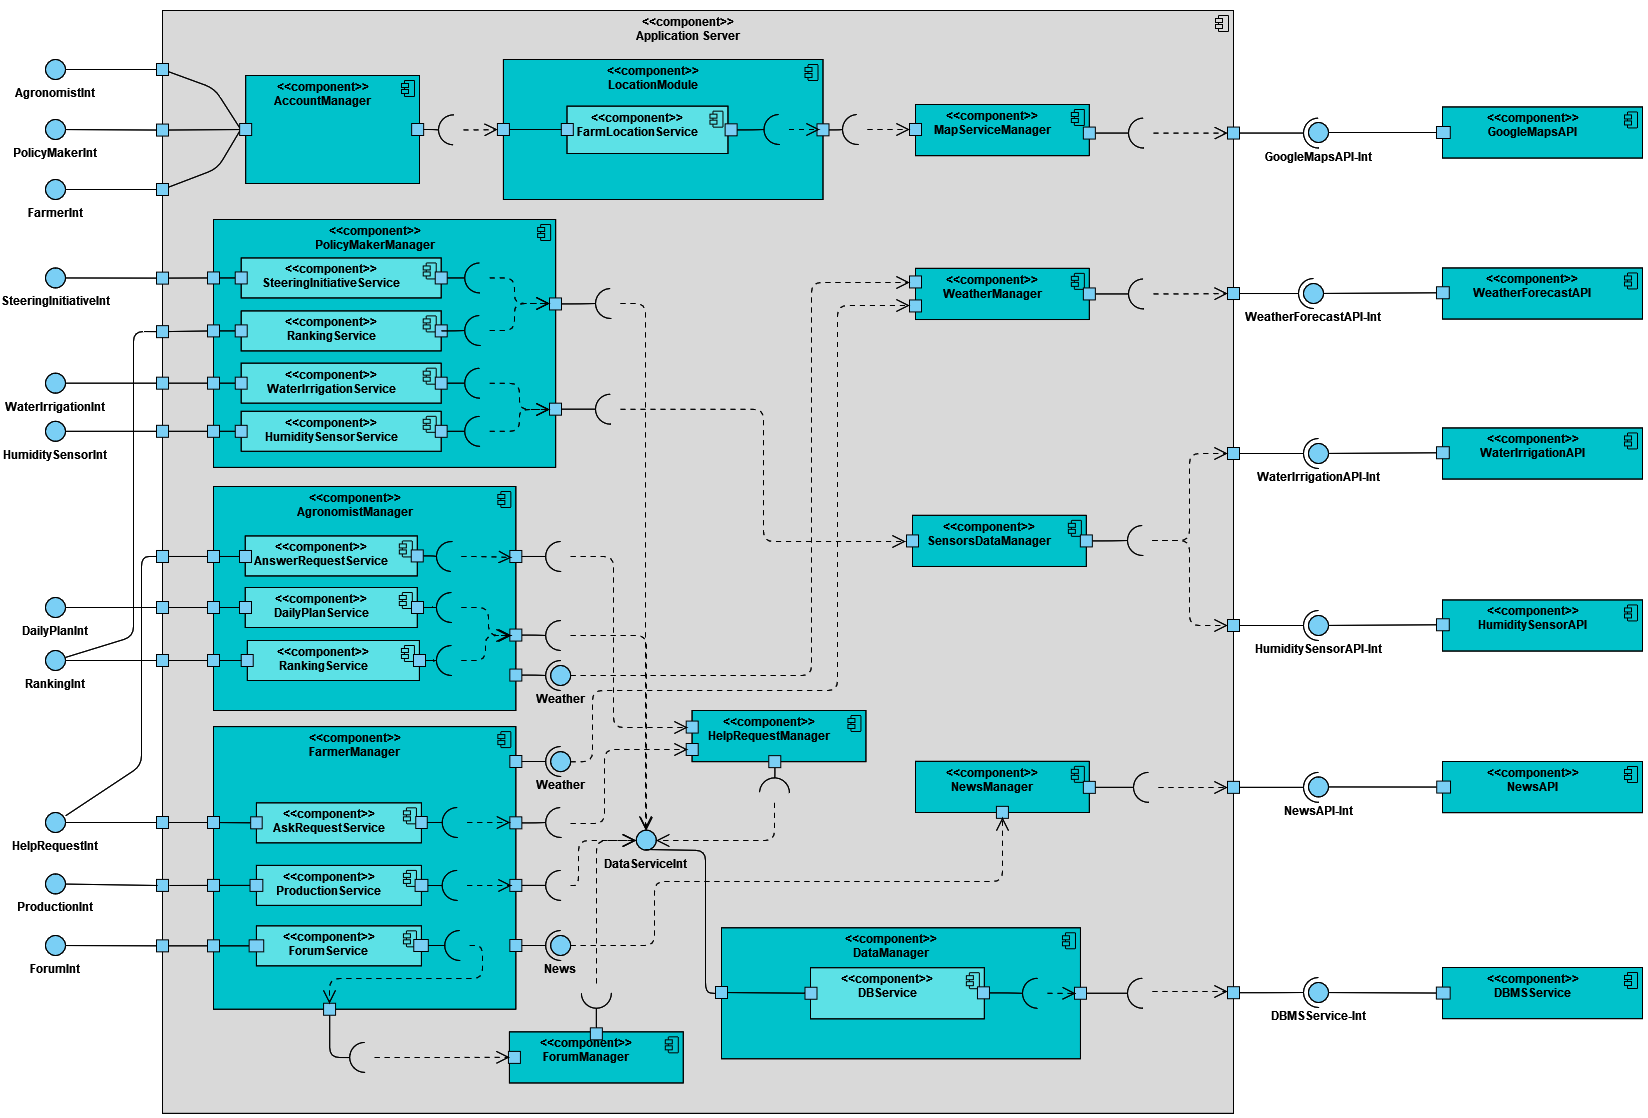
\includegraphics[scale=0.45, center]{assets/application-server-component.png}
        \caption{Application Server Component Diagram}
        \label{fig: application_server_component_view}
    \end{figure}
\end{center}

The following component diagram gives a detailed view of the Application Server. It shows the internal structure and the interaction between the components.
External elements in the diagram are represented in a simplified way.
\begin{itemize}
    \item \textbf{AccountManager}: this component handles all the basic requests made by the client.
    The \textit{AuthenticationService} manages the authentication process that is composed by the log in, the log out and the sign up services. 
    Once a user is logged in, all the specific functionalities are provided by the component that manages this type of user.
    \item \textbf{PolicyMakerManager}: it manages the policy maker services, these include: download of steering initiatives' reports submitted by agronomists, farmers' ranking, visualization of water irrigation sensors data and humidity sensors data.
    The steering initiative service and the ranking service are linked through an interface to the internal database, on the other side the water irrigation service and the humidity sensor service are considered external services and are managed by the \textit{SensorsDataManager}.
    \item \textbf{AgronomistManager}: it manages the agronomist services, these include: answer help requests, creation and updating of daily plans, farmers' ranking and uploading of steering initiatives.
    The daily plan service, the ranking service and the upload reports services are linked to the internal database, instead the answer request service communicates directly with the \textit{HelpRequestManager} component.
    \item \textbf{FarmerManager}: it manages the farmer services, these include: submit help requests, insert production data and participate in the forum.
    It includes one external interface that communicates with the \textit{NewsManager} component.
    In this case, only the production service is linked directly to the internal database, instead the ask request service is linked to the \textit{HelpRequestManager} component, while the forum service exposes an interface to connect to the \textit{ForumManager} component.
    \item \textbf{ForumManager}: this component manages the forum section, in particular it is responsible of the management of all the topics with the related messages between farmers.
    \item \textbf{DataManager}: it provides access to the external interface of the database, it manages queries and interacts with the DBMS.
    It includes one component that expose an interface that allow other internal components to communicate with the database.
    This component is connected to the \textit{DBMSService} external component, establishing the connection between the Application Server and the Database Server.
    \item \textbf{HelpRequestManager}: it manages the help requests between farmers and agronomists.
    It communicates with the \textit{FarmerManager} component for submitting a farmer's help request, on the other way it communicates with the \textit{AgronomistManager} component for the ones to answer. Essentially, it works as the dispatcher of messages between the two type of user.
    Finally, it provides an interface that communicates with the internal database in order to store the exchanged messages.
    \item \textbf{RankingManager}: it manages the ranking system for both the policy maker and the agronomist.
    It is responsible for calculating the final score used to compare the farmers in the ranking.
    More details on how to calculate it can be found in \textit{Section (\ref{other_design_decisions})}.
    \item \textbf{SteeringInitiativeManager}: it manages the steering initiatives for both agronomists and policy makers. It communicates with the \textit{AgronomistManager} in order to let the user write the report and with the \textit{PolicyMakerManager} in order to visualize it.
    \item \textbf{NewsManager}: this component manages the service related to the news, it provides updated suggestions about crops and fertilizers for the farmers.
    To do this, it interacts with the external component \textit{NewsService}.
    \item \textbf{SensorsDataManager}: this component handles two external APIs, the first one is provided by the water irrigation system and the other one provided by the humidity sensors.
    Both services are used by the \textit{PolicyMakerManager}.
\end{itemize}


\subsubsection*{Web Server Component View}
Regarding the Web Server the main components are:
\begin{itemize}
    \item \textbf{LocationModule}: this module provides the interface that allows the geolocalization of the farm based on the GPS (functionality available for farmer users) or on the address provided by the farmer.
    In order to provide this service, it communicates with the \textit{MapServiceManager}.
    \item \textbf{MapServiceManager}: this component communicates directly with the external API provided by \textit{Google Maps}, it provides information regarding the district and allows the user to visualize the map of a specific location.
    Mainly it adapts the data received by the API in a comprehensible way for the other components.
    \item \textbf{WeatherManager}: this component manages the service related to the weather forecast.
    It interacts with the external API provided by \textit{Open Weather} in order to get the weather data tailored to the user location.
\end{itemize}

\newpage
\subsection{Deployment view}
\begin{center}
    \begin{figure}[H]
        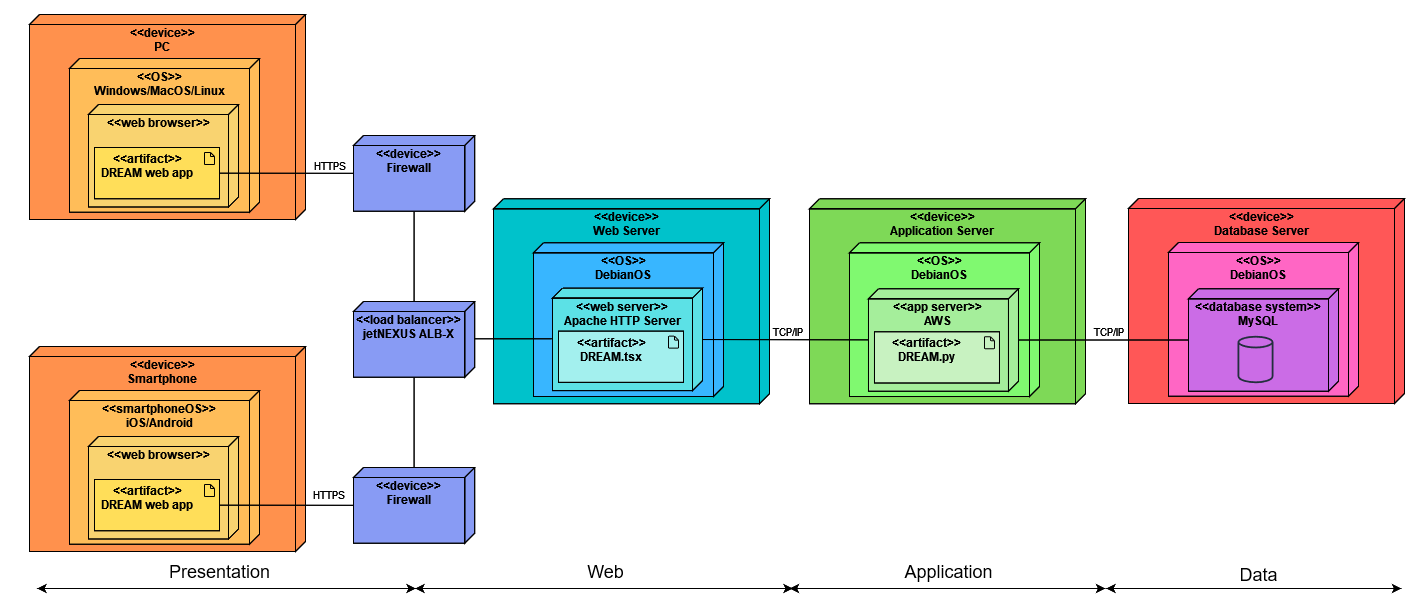
\includegraphics[scale=0.45, center]{assets/deployment_diagram.png}
        \caption{Deployment Diagram}
        \label{fig: deployment_diagram}
    \end{figure}
\end{center}

The deployment diagram in \textit{Figure (\ref{fig: deployment_diagram})} shows the most important components necessary for the correct behaviour of the system.
The devices shown in the diagram are:
\begin{itemize}
    \item \textbf{PC/Smartphone}: they are the client machines, they can be used by all the type of users.
    One allows the user to connect to the Web Server through a web browser as long as the HTTPS protocol is used.
    \item \textbf{Firewall}: first level of security, it guarantees safety access to the internal network of the system.
    \item \textbf{Load balancer}: the main goal is to prevent an overload of a server, this device distributes the incoming requests equally across multiple servers.
    This increase availability and reliability of the application.
    The one selected are the \textit{Heroku HTTP routers} provided by the hosting service. More details in section \ref{server_availability}.
    \item \textbf{Web Server}: it manages the HTTPS requests from the clients and route them to the \textit{Application Server} for processing.
    It is responsible of the incoming responses from the application server, they are managed by serving an HTML file to the client in addition to CSS and JS sheets.
    The result page is built with a client-side scripting.
    It also manages the external APIs such as the GoogleMapsAPI and the OpenWeatherAPI.
    Finally, web servers are duplicated to ensure high scalability and to guarantee good performance in case of a single point of failure.
    \item \textbf{Application Server}: it runs the core functionalities of the system, here there is the application logic.
    It also manages some external services such as the news, the water irrigation service and humidity service.
    Just like the \textit{Web Server}, for the same reasons, it is duplicated.
    Finally, it establishes the connection with the data tier through the DBMS interface. The \textit{Application Server} and the \textit{Database Server} are connected through an internal LAN, there are no firewalls between them in order to increase the average connection speed.

    \item \textbf{Database Server}: it represents the data tier, it receives the data insertions and data queries from the \textit{Application Server} and manages them.
    PostgreSQL has been selected as the main database infrastructure, this allows to easily manage in a secure way the data storage and requests.
    
\end{itemize}
\newpage
\subsection{Runtime view}

Here the runtime views of some relevant use cases of the system are represented through sequence diagrams. 
In the diagrams, the part regarding the user is omitted because it has been deemed as redundant to the understanding of the interaction.
In later diagrams, some parts, like the login phase or returning to home page, were omitted for the the same motivations.

\newpage
\textbf{Sign Up}
\begin{center}
    \begin{figure}[H]
        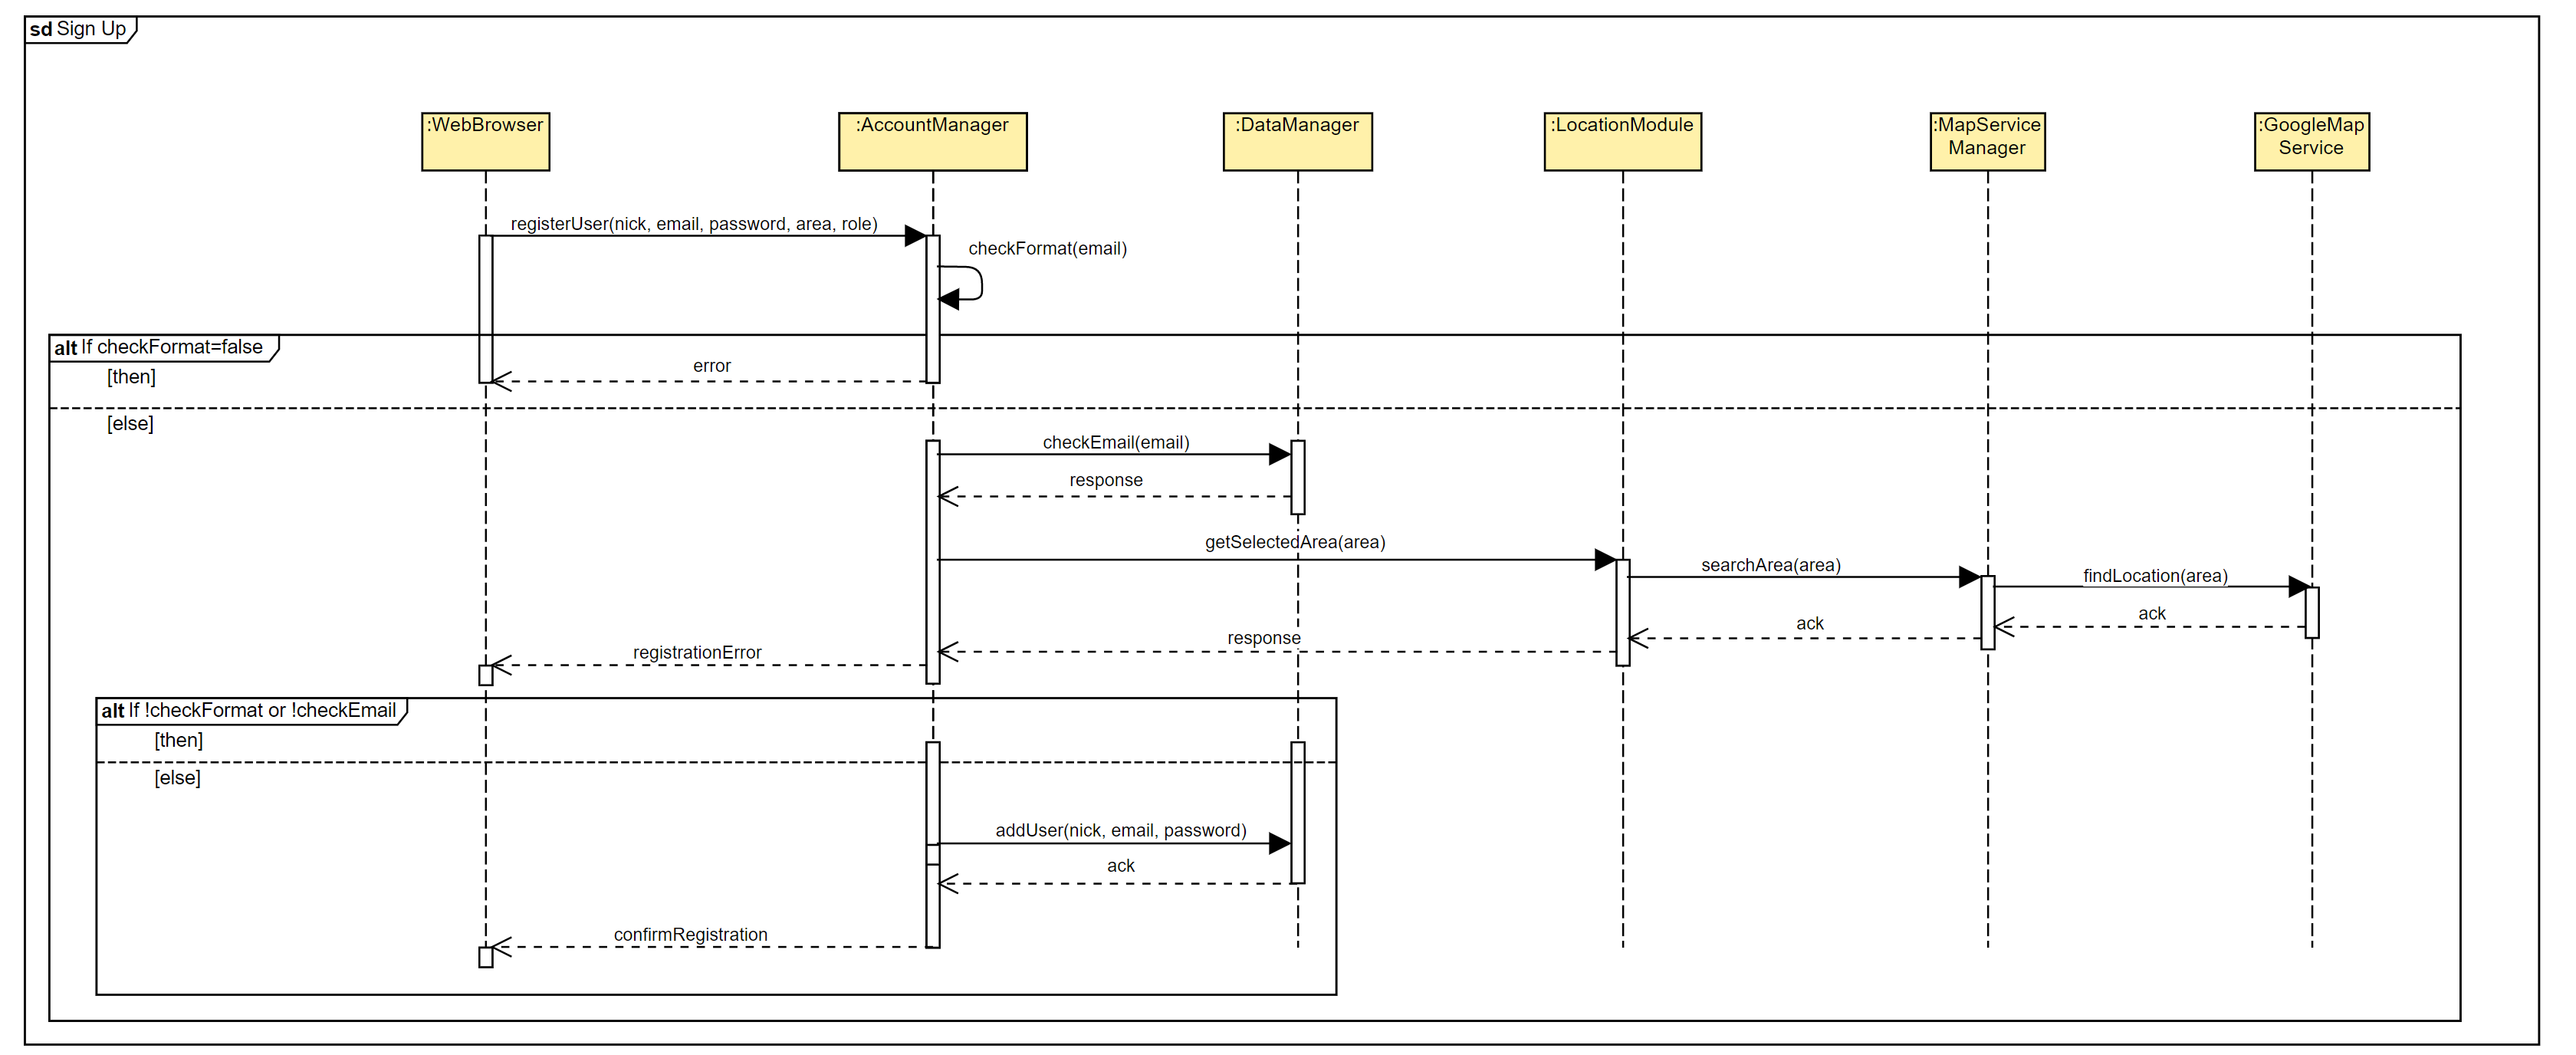
\includegraphics[scale=0.67, center]{assets/SequenceDiagram/SignUp.png}
        \caption{Sign Up}
        \label{fig:signup}
    \end{figure}
\end{center}
Sign up is pretty standard: user registers himself/herself by inserting first name, last name, email, password, job role and district (if the user isn't a Policy Maker).
If the user is a farmer, in a following page, he/she chooses also the crop type the farm deals with.
Farmer can select manually their address without the use of GPS.

At the end of the process, if every check results successful, the user is registered to the database by the \textit{DataManager} component.

\newpage
\textbf{Log In}
\begin{center}
    \begin{figure}[H]
        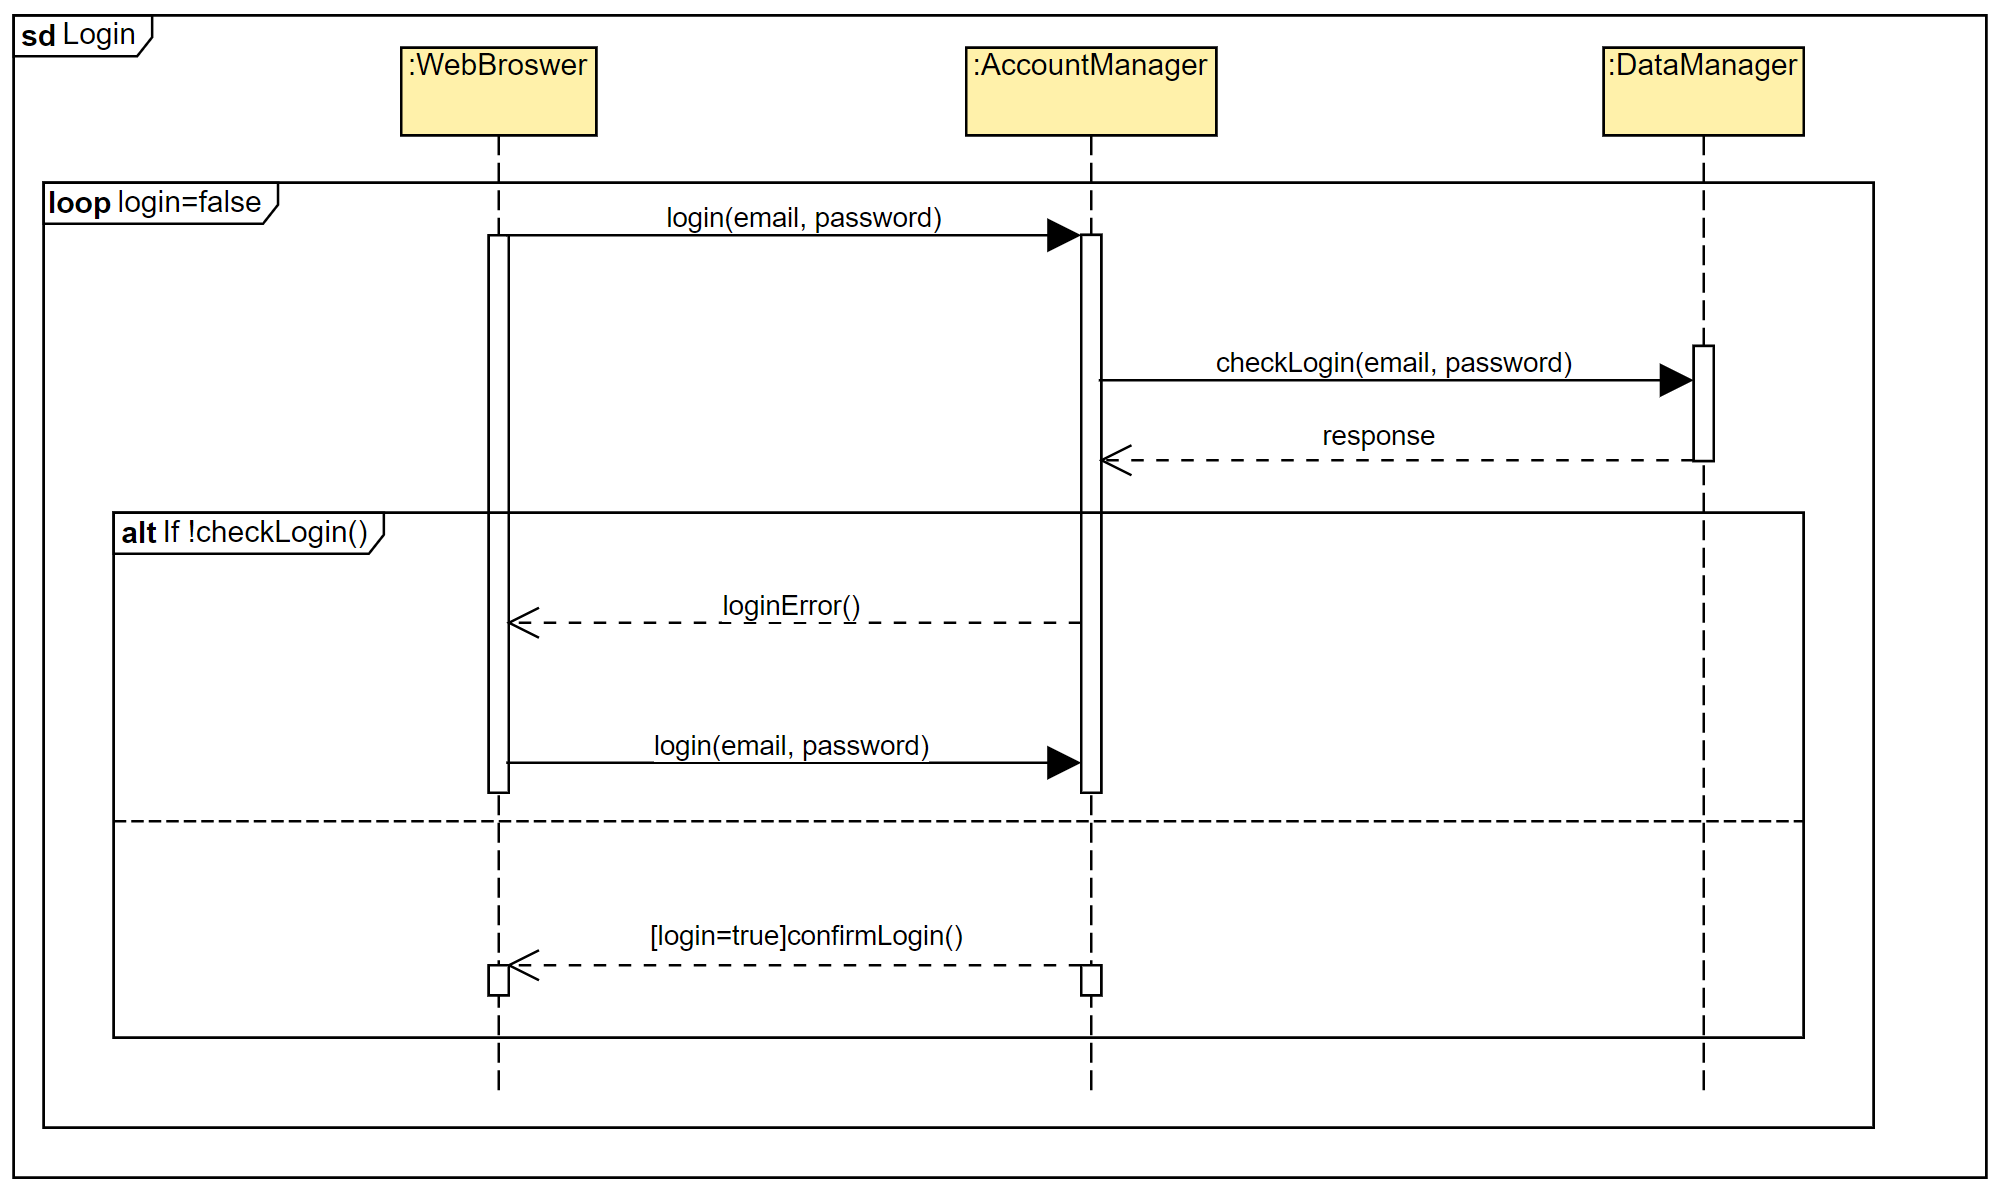
\includegraphics[scale=0.8, center]{assets/SequenceDiagram/Login.png}
        \caption{Log In}
        \label{fig: login}
    \end{figure}
\end{center}

The Log In phase simply consists in the user action of inserting their email (unique key in the database) and password in the login fields, then the system checks if the pair corresponds to a user entry in the database.
In case of success, the user can log in the system and use its functionalities available for that particular type of account chosen during the Sign Up phase.

\newpage
\textbf{View Steering Initiative Reports}
\begin{center}
    \begin{figure}[H]
        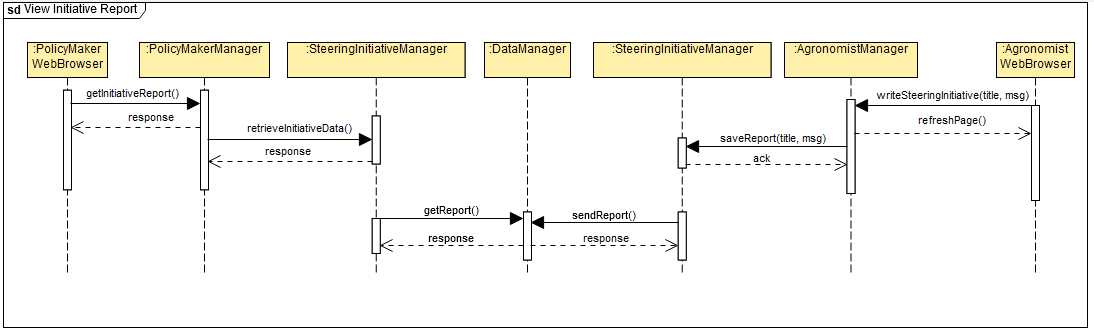
\includegraphics[scale=0.70, center]{assets/SequenceDiagram/ViewInitiativeReport.png}
        \caption{View Initiative Report}
        \label{fig: report}
    \end{figure}
\end{center}
This sequence diagram represents the interactions between components that occur when displaying the steering initiatives (previously uploaded in the database by agronomists) to a policy maker user.

\newpage
\textbf{Check Soil Humidity Data}
\begin{center}
    \begin{figure}[H]
        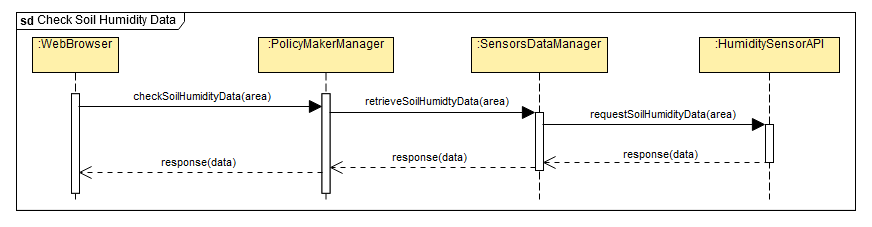
\includegraphics[scale=0.80, center]{assets/SequenceDiagram/CheckSoilHumidityData.png}
        \caption{Check Soil Humidity Data}
        \label{fig: humidity}
    \end{figure}
\end{center}
This sequence diagram represents the interactions between components that occur when displaying the sensors data regarding soil humidity to a policy maker user.
The business logic running on the Application Server retrieves these data from an external source, furthermore it handles them just temporarily since they are not modified by the \textit{DREAM} system and they're fetched on user demand.

\newpage
\textbf{Check Water Irrigation Data} 
\begin{center}
    \begin{figure}[H]
        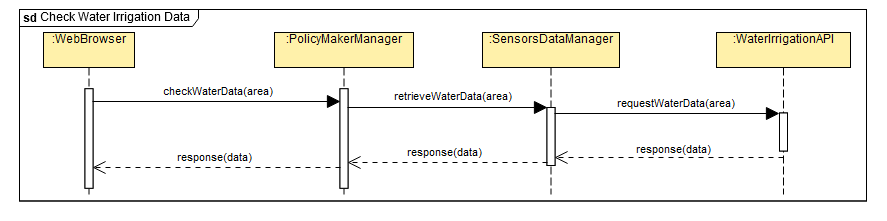
\includegraphics[scale=0.80, center]{assets/SequenceDiagram/CheckWaterIrrigationData.png}
        \caption{Check Water Irrigation Data}
        \label{fig: irrigation}
    \end{figure}
\end{center}
This sequence diagram represents the interactions between components that occur when displaying the sensors data regarding the water irrigation to a policy maker user.
The function is the same of the above mentioned case.

\newpage
\textbf{View Farmers Ranking}
\begin{center}
    \begin{figure}[H]
        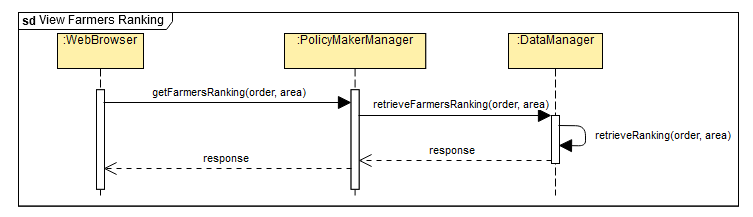
\includegraphics[scale=0.85, center]{assets/SequenceDiagram/ViewFarmersRanking.png}
        \caption{View Farmers Ranking}
        \label{fig: ranking}
    \end{figure}
\end{center}
This sequence diagram represents the interactions between components that occur when displaying the farmers ranking to policy maker and agronomist users.
It will be explained better later in the document. %add \ref{}
The function includes an area parameter to specify of which area the user wants the ranking.
In order to achieve code reusability, this function is invoked by either policy makers or agronomists. 
When a policy maker wants to see the ranking the parameter \texttt{area} will be set to \texttt{all} in order to obtain the ranking comprehensive of all Telangana's farmer registered in the app.
Instead, when an agronomist wants to use this functionality, \texttt{area} will be automatically taken to his/her respective responsibility area. By doing this, the function becomes more modular.

\newpage
\textbf{View Specific Farmers Informations}
\begin{center}
    \begin{figure}[H]
        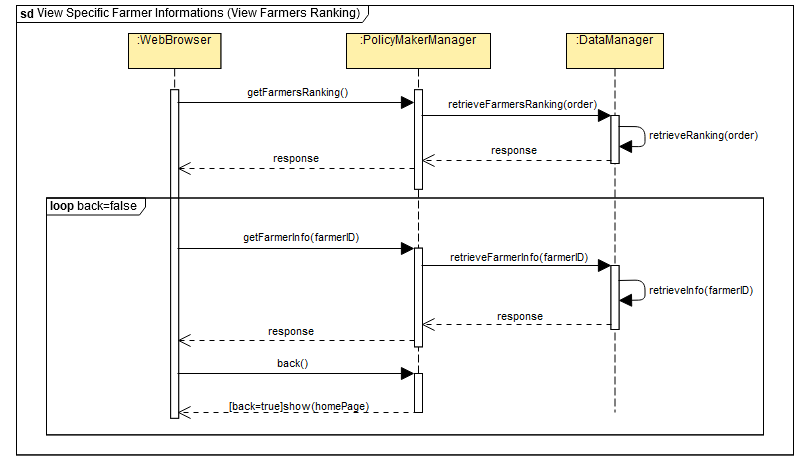
\includegraphics[scale=0.8, center]{assets/SequenceDiagram/ViewSpecificFarmerInformations.png}
        \caption{View Specific Farmer Informations}
        \label{fig: specificFarmerInfo}
    \end{figure}
\end{center}
This sequence diagram represents the interactions between components caused by a search for a specific farmer information summary.

\newpage
\textbf{Insert Production Data}
\begin{center}
    \begin{figure}[H]
        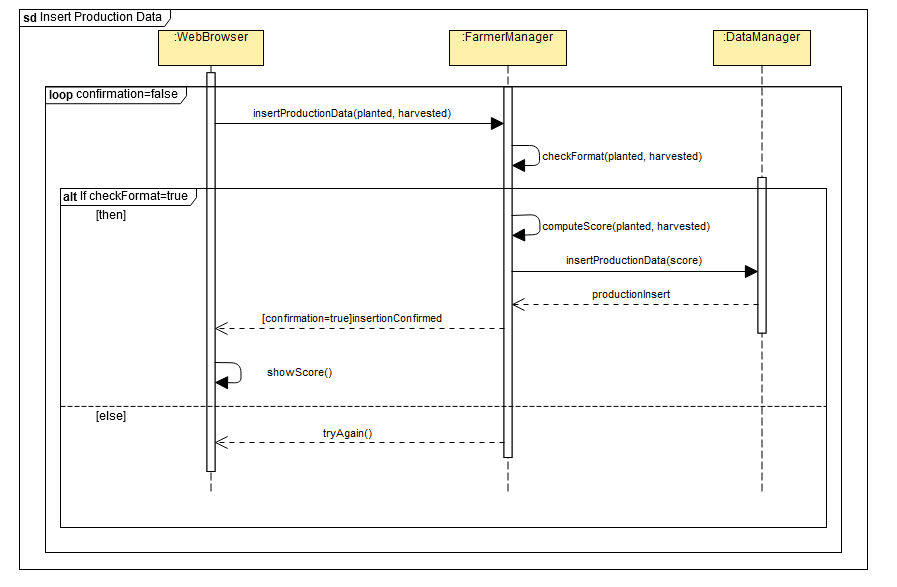
\includegraphics[scale=0.75, center]{assets/SequenceDiagram/InsertProductionData.png}
        \caption{Insert Production Data}
        \label{fig: production}
    \end{figure}
\end{center}
This sequence diagram represents the interactions between components caused by an insertion of production data from a farmer user.
Each new production entry cause the score associated to the farmer to be calculated again and updated. So the score shall be an attribute of each farmer profile. Since a farmer's rank is directly proportionated to the his/her score, the recomputation can lead to a shifting in the general ranking too.

\newpage
\textbf{Check News}
\begin{center}
    \begin{figure}[H]
        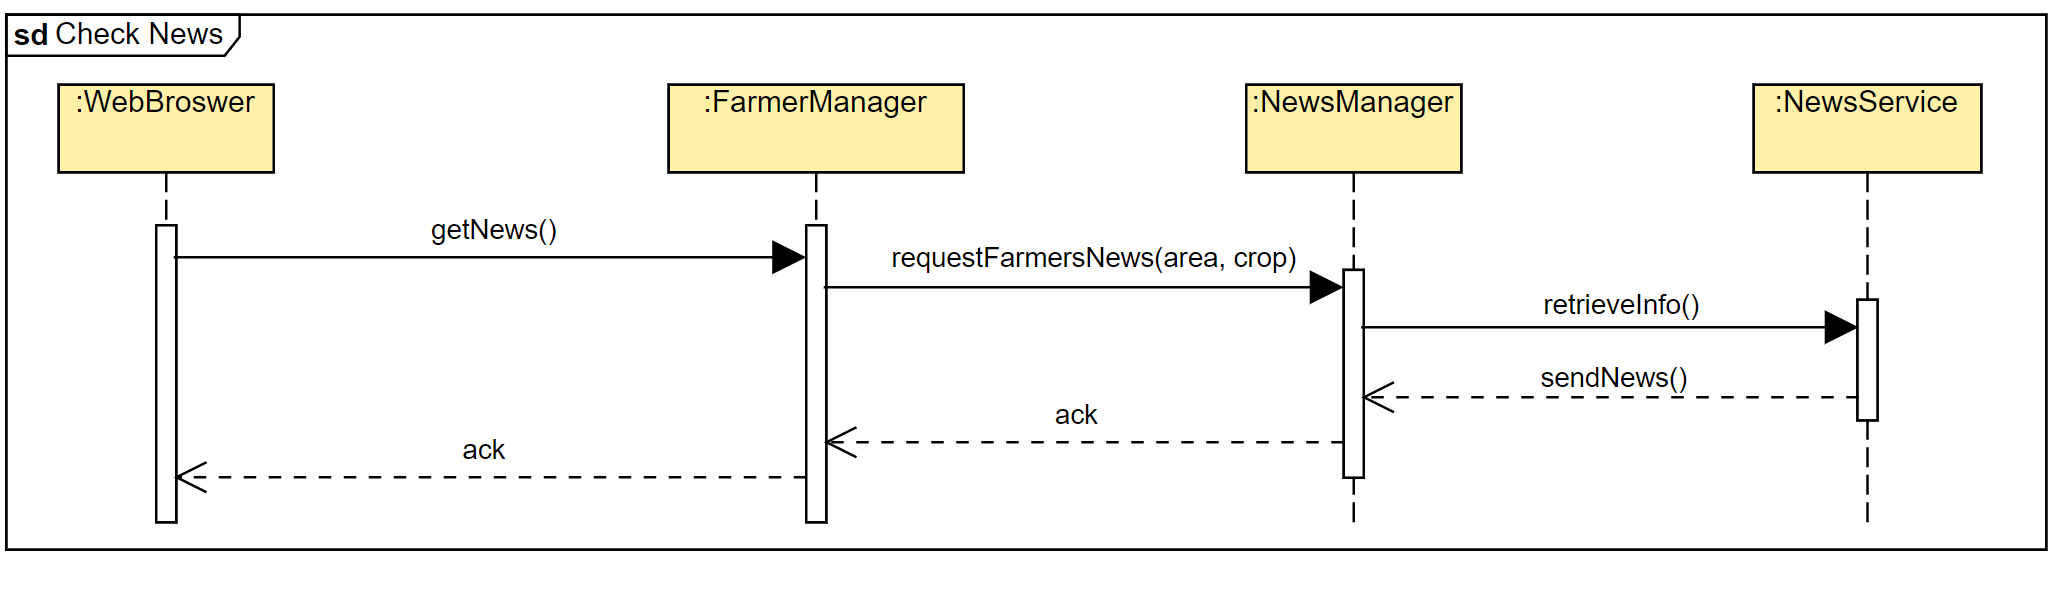
\includegraphics[scale=0.6, center]{assets/SequenceDiagram/CheckNews.png}
        \caption{Check News}
        \label{fig: news}
    \end{figure}
\end{center}
This sequence diagram represents the interactions between components that occur when displaying the news regarding farmers' interests to them, such as news concering the same area or crop type of the farmer.
The \textit{NewsManager} uses the \textit{NewsAPI} component in order to get always up-to-date news.

\newpage
\textbf{Forum}
\begin{center}
    \begin{figure}[H]
        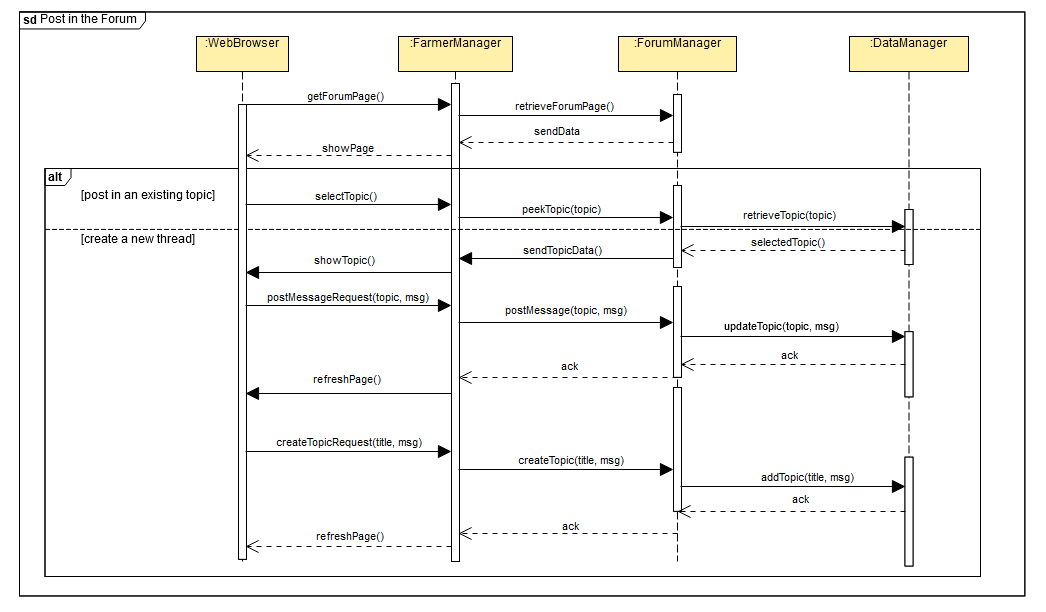
\includegraphics[scale=0.5, center]{assets/SequenceDiagram/PostInTheForum.png}
        \caption{Forum}
        \label{fig: forum}
    \end{figure}
\end{center}
This sequence diagram represents the interactions between the components of the forum. 
It is split into two part: the one that allows the user to make a post in an already existing topic and the one that allows the user to create a new topic.

\newpage
\textbf{Check Weather Forecast}
\begin{center}
    \begin{figure}[H]
        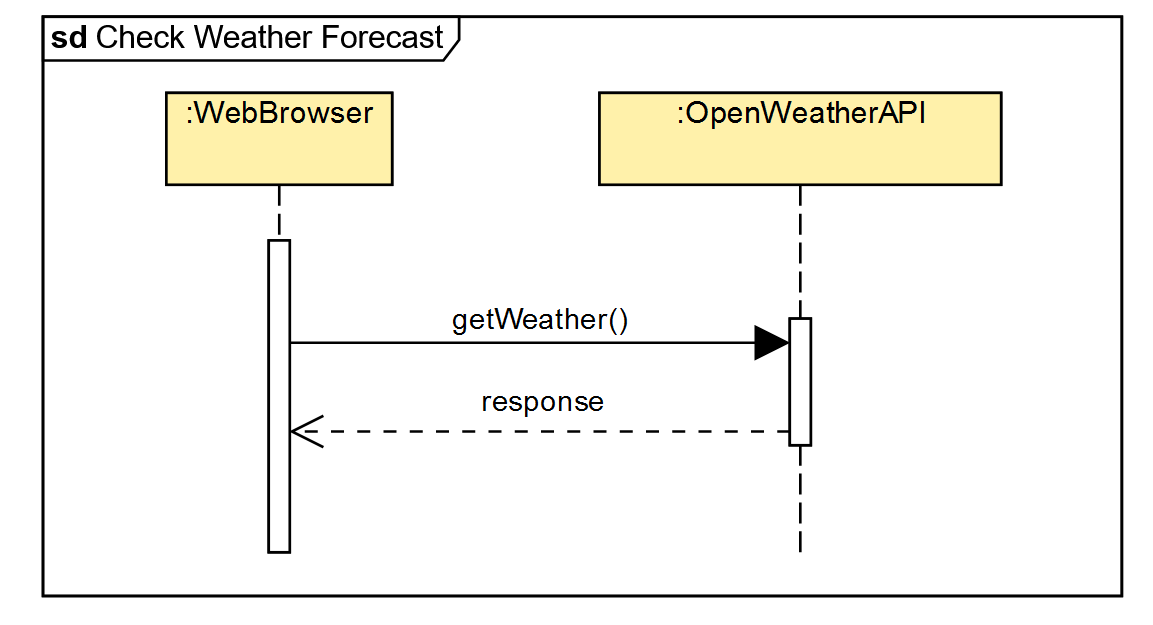
\includegraphics[scale=0.6, center]{assets/SequenceDiagram/CheckWeatherForecast.png}
        \caption{Check Weather Forecast}
        \label{fig: forecast}
    \end{figure}
\end{center}
This sequence diagram represents the interactions between components that occur when displaying the weather forecast to the users. The weather report is tailored to the user area.
The \textit{WeatherManager} component uses the \textit{OpenWeatherAPI} component in order to get always up-to-date forecast.

\newpage
\textbf{Help Request}
\begin{center}
    \begin{figure}[H]
        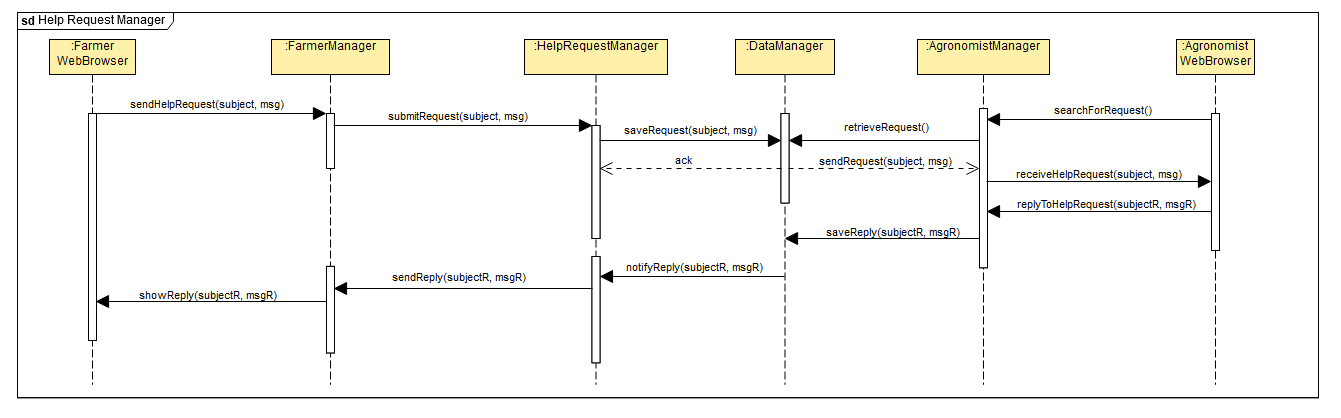
\includegraphics[scale=0.55, center]{assets/SequenceDiagram/HelpRequestManager.png}
        \caption{Help Request}
        \label{fig: helpRequest}
    \end{figure}
\end{center}
This sequence diagram represents the interactions between the components needed to manage the help requests that the farmers send to the agronomists.
When a farmer sends an help request, the system saves it in the database.
When the agronomist is online, the system checks if there are some unread messages in the database and sends them to the agronomist.
The agronomist replies to the request and saves it into the database. 
When the farmer is online the system checks if there are some unread replies in the database and displays them to the farmer.
Since the exchange is necessarily asynchronous because of the fact that the receiver of the message might be offline in the moment of the delivery, the messages have to be stored on the database and the unread ones have to be fetched each time the user is back online.

\newpage
\textbf{Daily Plan Management}
\begin{center}
    \begin{figure}[H]
        
        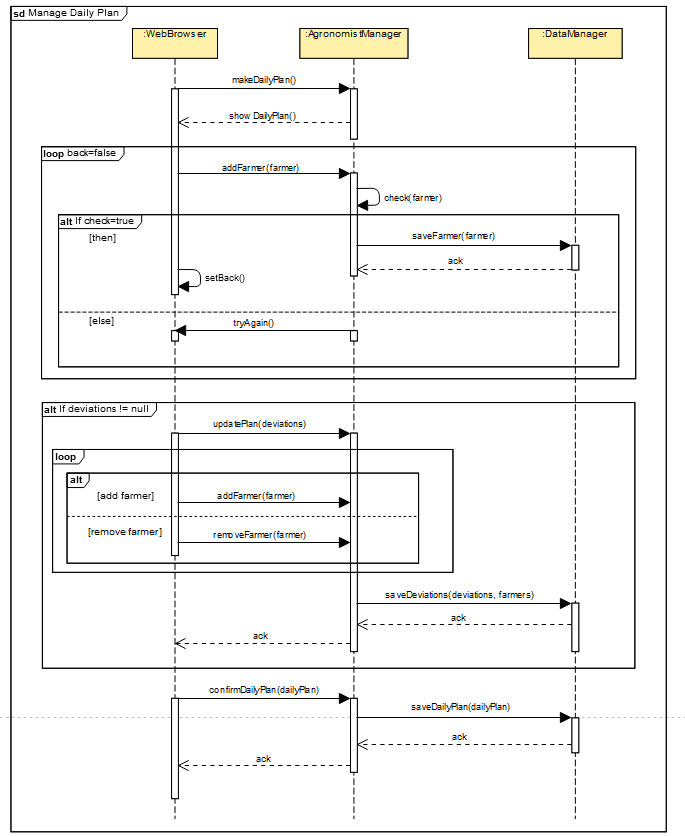
\includegraphics[scale=0.70, center]{assets/SequenceDiagram/ManageDailyPlan.png}
        \caption{Daily Plan}
        \label{fig: dailyPlan}
    \end{figure}
\end{center}
This sequence diagram represents the interactions between components in managing the daily plan.
In the diagram, there are both the creation and the updating of the daily plan.

\newpage
\textbf{Upload Steering Initiative}
\begin{center}
    \begin{figure}[H]
        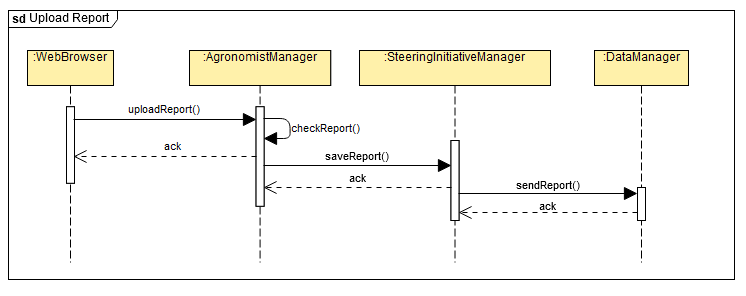
\includegraphics[scale=0.7, center] {assets/SequenceDiagram/uploadReport.png}
        \caption{Upload Report}
        \label{fig: uploadReport}
    \end{figure}
\end{center}
This sequence diagram represents the interactions between components in managing the uploading of the Steering Initiative.

\newpage
\subsection{Component interfaces}

\begin{center}
    \begin{figure}[H]
        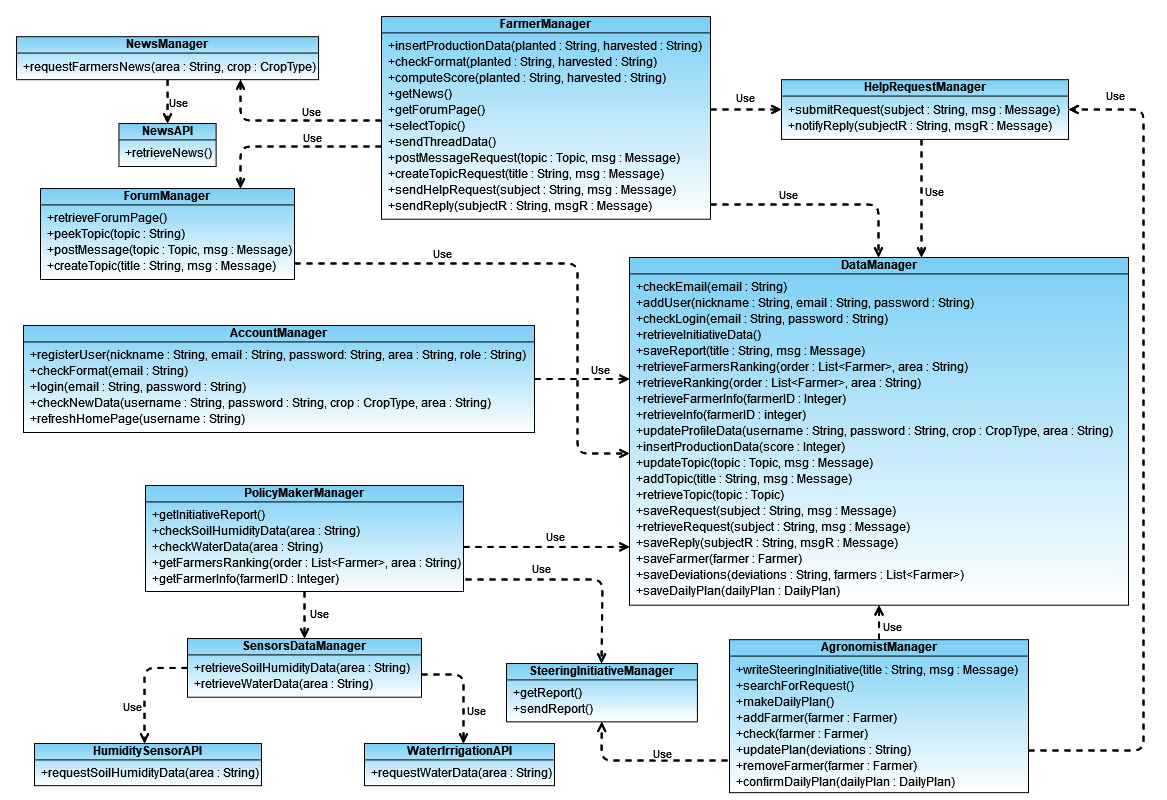
\includegraphics[scale=0.60, center]{assets/component-interfaces.png}
        \caption{Component Interfaces Diagram}
        \label{fig: component_interfaces}
    \end{figure}
\end{center}

This diagram above describes in detail the interfaces and the corresponding methods offered by each component, it also shows the interaction between them.
The diagram refers to the component diagrams in \textit{Figure (\ref{fig: general_component_view})} and \textit{Figure (\ref{fig: application_server_component_view})}.
Please note that the methods described in \textit{Figure (\ref{fig: component_interfaces})} don't represent exactly the final version that will be used during the implementation, they just provide a logical representation.

\subsection{Selected architectural styles and patterns}

    \begin{itemize}
        \item \textbf{Four tier architecture} \newline
              This kind of architecture divides the system in four different modules: client, presentation, applications and data tier.
              As descibed in the previous sections, the architecture is based on this architectural style.
        \item \textbf{Thin client} \newline
              The thin client approach increases performance and security since every piece of data and business logic code are not stored locally but in a server.
        \item \textbf{Scalability} \newline
              A four tiers application guarantees that a scaling architecture approach is adopted only for the most critical components.
              The result obtained maximize the performances but also minimize the costs.
        \item \textbf{Model View Controller} \newline
              Model-View-Controller \cite{mvc} (MVC) is a software design pattern used for developing user interfaces that divides the program logic into three interconnected elements.
              This separate internal information representations from the ways they're presented to and accepted from the user.
              These three components are:
              \begin{itemize}
                  \item Model: the central component of the pattern. It is the application's dynamic data structure, independent of the user interface. It directly manages the data, logic and rules of the application.
                  \item View: The view defines how the app's data should be displayed.
                  \item Controller: it contains logic that updates the model and/or view in response to input from the users of the app. 
              \end{itemize}
    \end{itemize}

\newpage

\subsection{Other design decisions}
\label{other_design_decisions}
\subsubsection{Servers availability and response time} 
\label{server_availability}
In order to guarantee the availability of 99.998\% promised in the RASD, replicas of the web servers and the application servers are needed, this prevents the system to crash in case of a point failure.
Servers replication is done by the hosting service Heroku.
The response time described in the RASD is 0.5 seconds, the load balancer will allow to reach this goal by distributing the incoming requests from users among the replicas.
The database server is replicated as well for the same reasons.
So that, in case of failure the system can continue to work, thanks to the distributed nature of the system. 

Furthermore, in case of failure of the whole system, the status can be restored thanks to backups. 
So a backup routine has to be planned.
Periodically, in an automated way, the system shall perform a backup of the system and replace the older copy with it.
\subsubsection{Farmers ranking} 
The ranking system has been thought as an aid for policy makers and agronomists to understand how the farmers are performing. However, there are multiple factors that play a role in a farmer's performance, some of them might be difficult to quantify. Furthermore, DREAM should highlight the climate resiliance aspects, which is not a trivial task.

In the first version of the app, the following formula is proposed in order to achieve a fair and scientific way to compute the score associated to each farmer.
\begin{equation}
    score = {harvested\ qty\over sown\ qty}\cdot \left( 1 + {hostile\ weather\ days\over 365}\right)
\end{equation}

The formula can be broken down into two parameters, $\eta$ and $\delta$:

\begin{align}  
    \eta &= {harvested\ qty\over sown\ qty}\\
    \delta &= {hostile\ weather\ days\over 365}
\end{align}
$\eta$ is the main term that represents the productivity of a farmer, that is how efficient he/she has been given the quantity of sown seeds (in kilograms) and the return in harvested crop (in kilograms). The data taken into consideration for $\eta$'s computation is the one collected in 12 months, from March to March of the previous year year\footnotemark, resetting the score to 0 every March.
In the computation, only full production entries (with an harvested quantity of the crop) are taken into consideration.

\footnotetext{March has been chosen as the reset month after comparing the sowing to harvesting period of all the most popular crop grown in India. In a solar year, the first to be sown are cucumbers and pumpkin, to the last to be harvested are wheat and mustard, all of these in March.} 

Whereas $\delta$ weighs up the harshness of the climate conditions endured by the farmer in the last year. The variable $hostile\ weather\ days$ is a counter of the days in which the climate has not been very lenient in the farm's region and could have ruined the plantation. Days are considered "hostile weather days" in case the amount of rain fallen during that day has been greater than 115.60 mm/hour (so in condition of very heavy rainfall or worse)\cite{rainfallsData}, particularly expected during monsoon seasons; as well as strong heat waves and prolonged periods of drought. Also specific crop disease that might have afflicted the region for a certain time during the year may be considered as challenging days to take in consideration. However, at the time of this document, just rainfalls data are available for the DREAM app, so only heavy rain days will be taken into account in computing the $\delta$ parameter.

The role of $\delta$ is to favor farmers that have been particularly hitten by climatic problems but still have managed to produce, since this demonstrate that they've been able to carry out usefull practices that helped them staying productive despite the natural adversities. 

A new $\delta$ parameter is computed everyday, for each one of the 10 Telangana's district. The $\delta$ is valid for just that day and is computed collecting all the data from today till the 12 months prior, creating a sliding window of a solar year. 

An upgrade of a farmer's production entry into a full one triggers the recomputation of their score, since their $\eta$ parameter changed. The new score will be affected by their district's $\delta$ computed that particular day in which the score has been triggered.

\begin{testexample}
Let's suppose it's the 15th of June and farmer Pajeet (in Medak district) has been using DREAM for 3 months. He inserts just one production entry stating that he has sown 10kg of rice the 15th of June in his land. His score is 0 since no full production entry has been inserted, that is the entry of Pajeet is still missing the harvested amount since the crop has not been harvested yet. From January to May, there have been several days of heavy rain, 23 days to be specific.

After five months, Pajeet harvests his rice field that has produced 10000kg of rice, so he upgrade the rice production entry (begun the 15/06) on his profile the 15th of November. This insertion cause his score to be recomputed because now the status of his rice prodcution entry has become "full". Since June, there have been 8 days of very heavy rainfalls in Medak: 7 days in Septemper and 1 day the 20th of October. Up to the 15th of November the $\delta$ parameter for Medak district is $\delta_{year}=\frac{23+8}{365}=0.085$. His score is updated the 15th Nov as follow: $score_{year}=\frac{10000}{10}(1+0.085)=1085$.

The 27-28th of November, it rains heavily in Medak again. The 29th of November, the policy maker Chaytanya queries the farmer ranking. There is Pajeet in the ranking, his score is still 1085.
\end{testexample}

 The rank is directly proportional to the farmer's current score. If farmers obtain the same score, they are going to be ranked in the same position as well.

\subsubsection{Farmers location} In order to locate a farm the user has two options:
    \begin{itemize}
        \item Address: farm can be located through the address inserted by the user during the sign up phase.
        The address is verified by the \textit{LocationModule}.
        \item GPS coordinates: if the address hasn't been inserted by the user or, if the \textit{LocationModule} doesn't find the address, the user can manually specify the coordinates with the help of the \textit{MapServiceManager}.
    \end{itemize}

\subsubsection{Agronomist daily plan} An agronomist can have at most one daily plan per day.
During the daytime it can be manually updated until the end of the visit day, when the system is going to automatically confirm the plan. If the agronomist doesn't manage to visit any of the farms planned for a day, he/she can update the plan and remove all the farmers from it so that it is going to be delete it from the database.

\newpage
\section{User Interface Design}
\begin{center}
    \begin{figure}[H]
        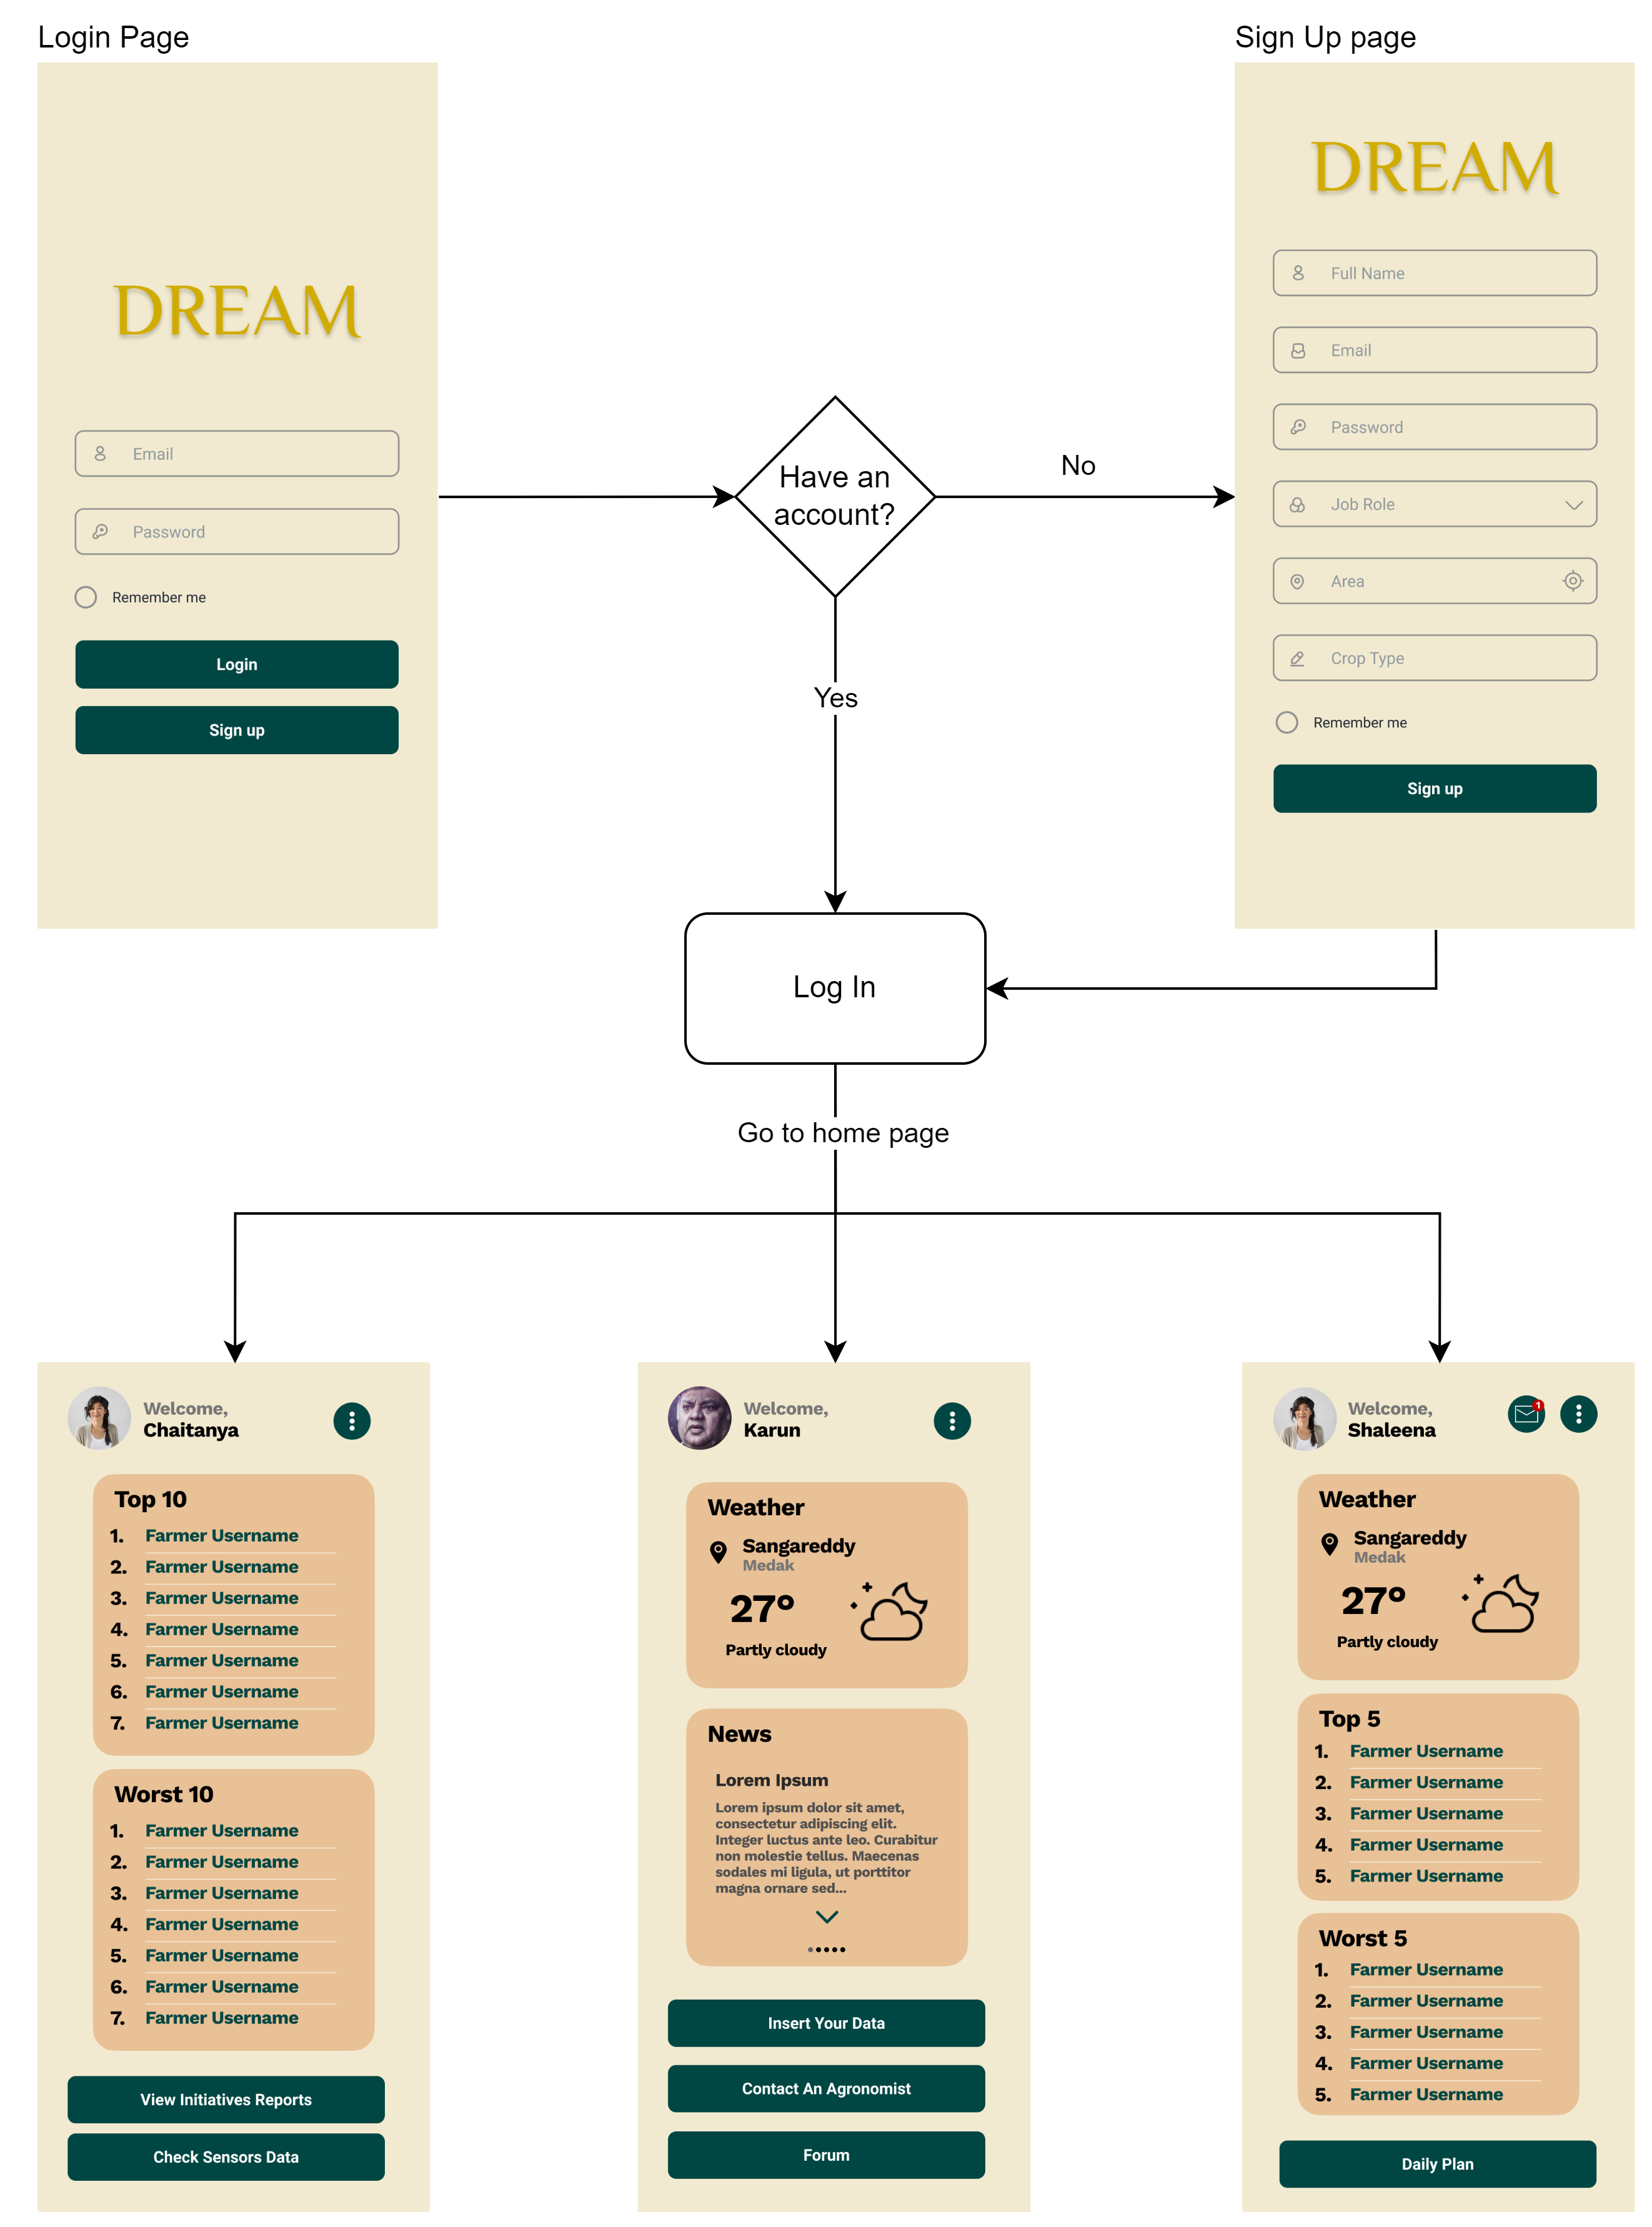
\includegraphics[scale=0.74, center]{assets/MockUp/SignUpandLogin.png}
        \caption{Sign Up and Log In}
        \label{fig: signMockup}
    \end{figure}
\end{center}

\begin{center}
    \begin{figure}[H]
        \vspace{-50px}
        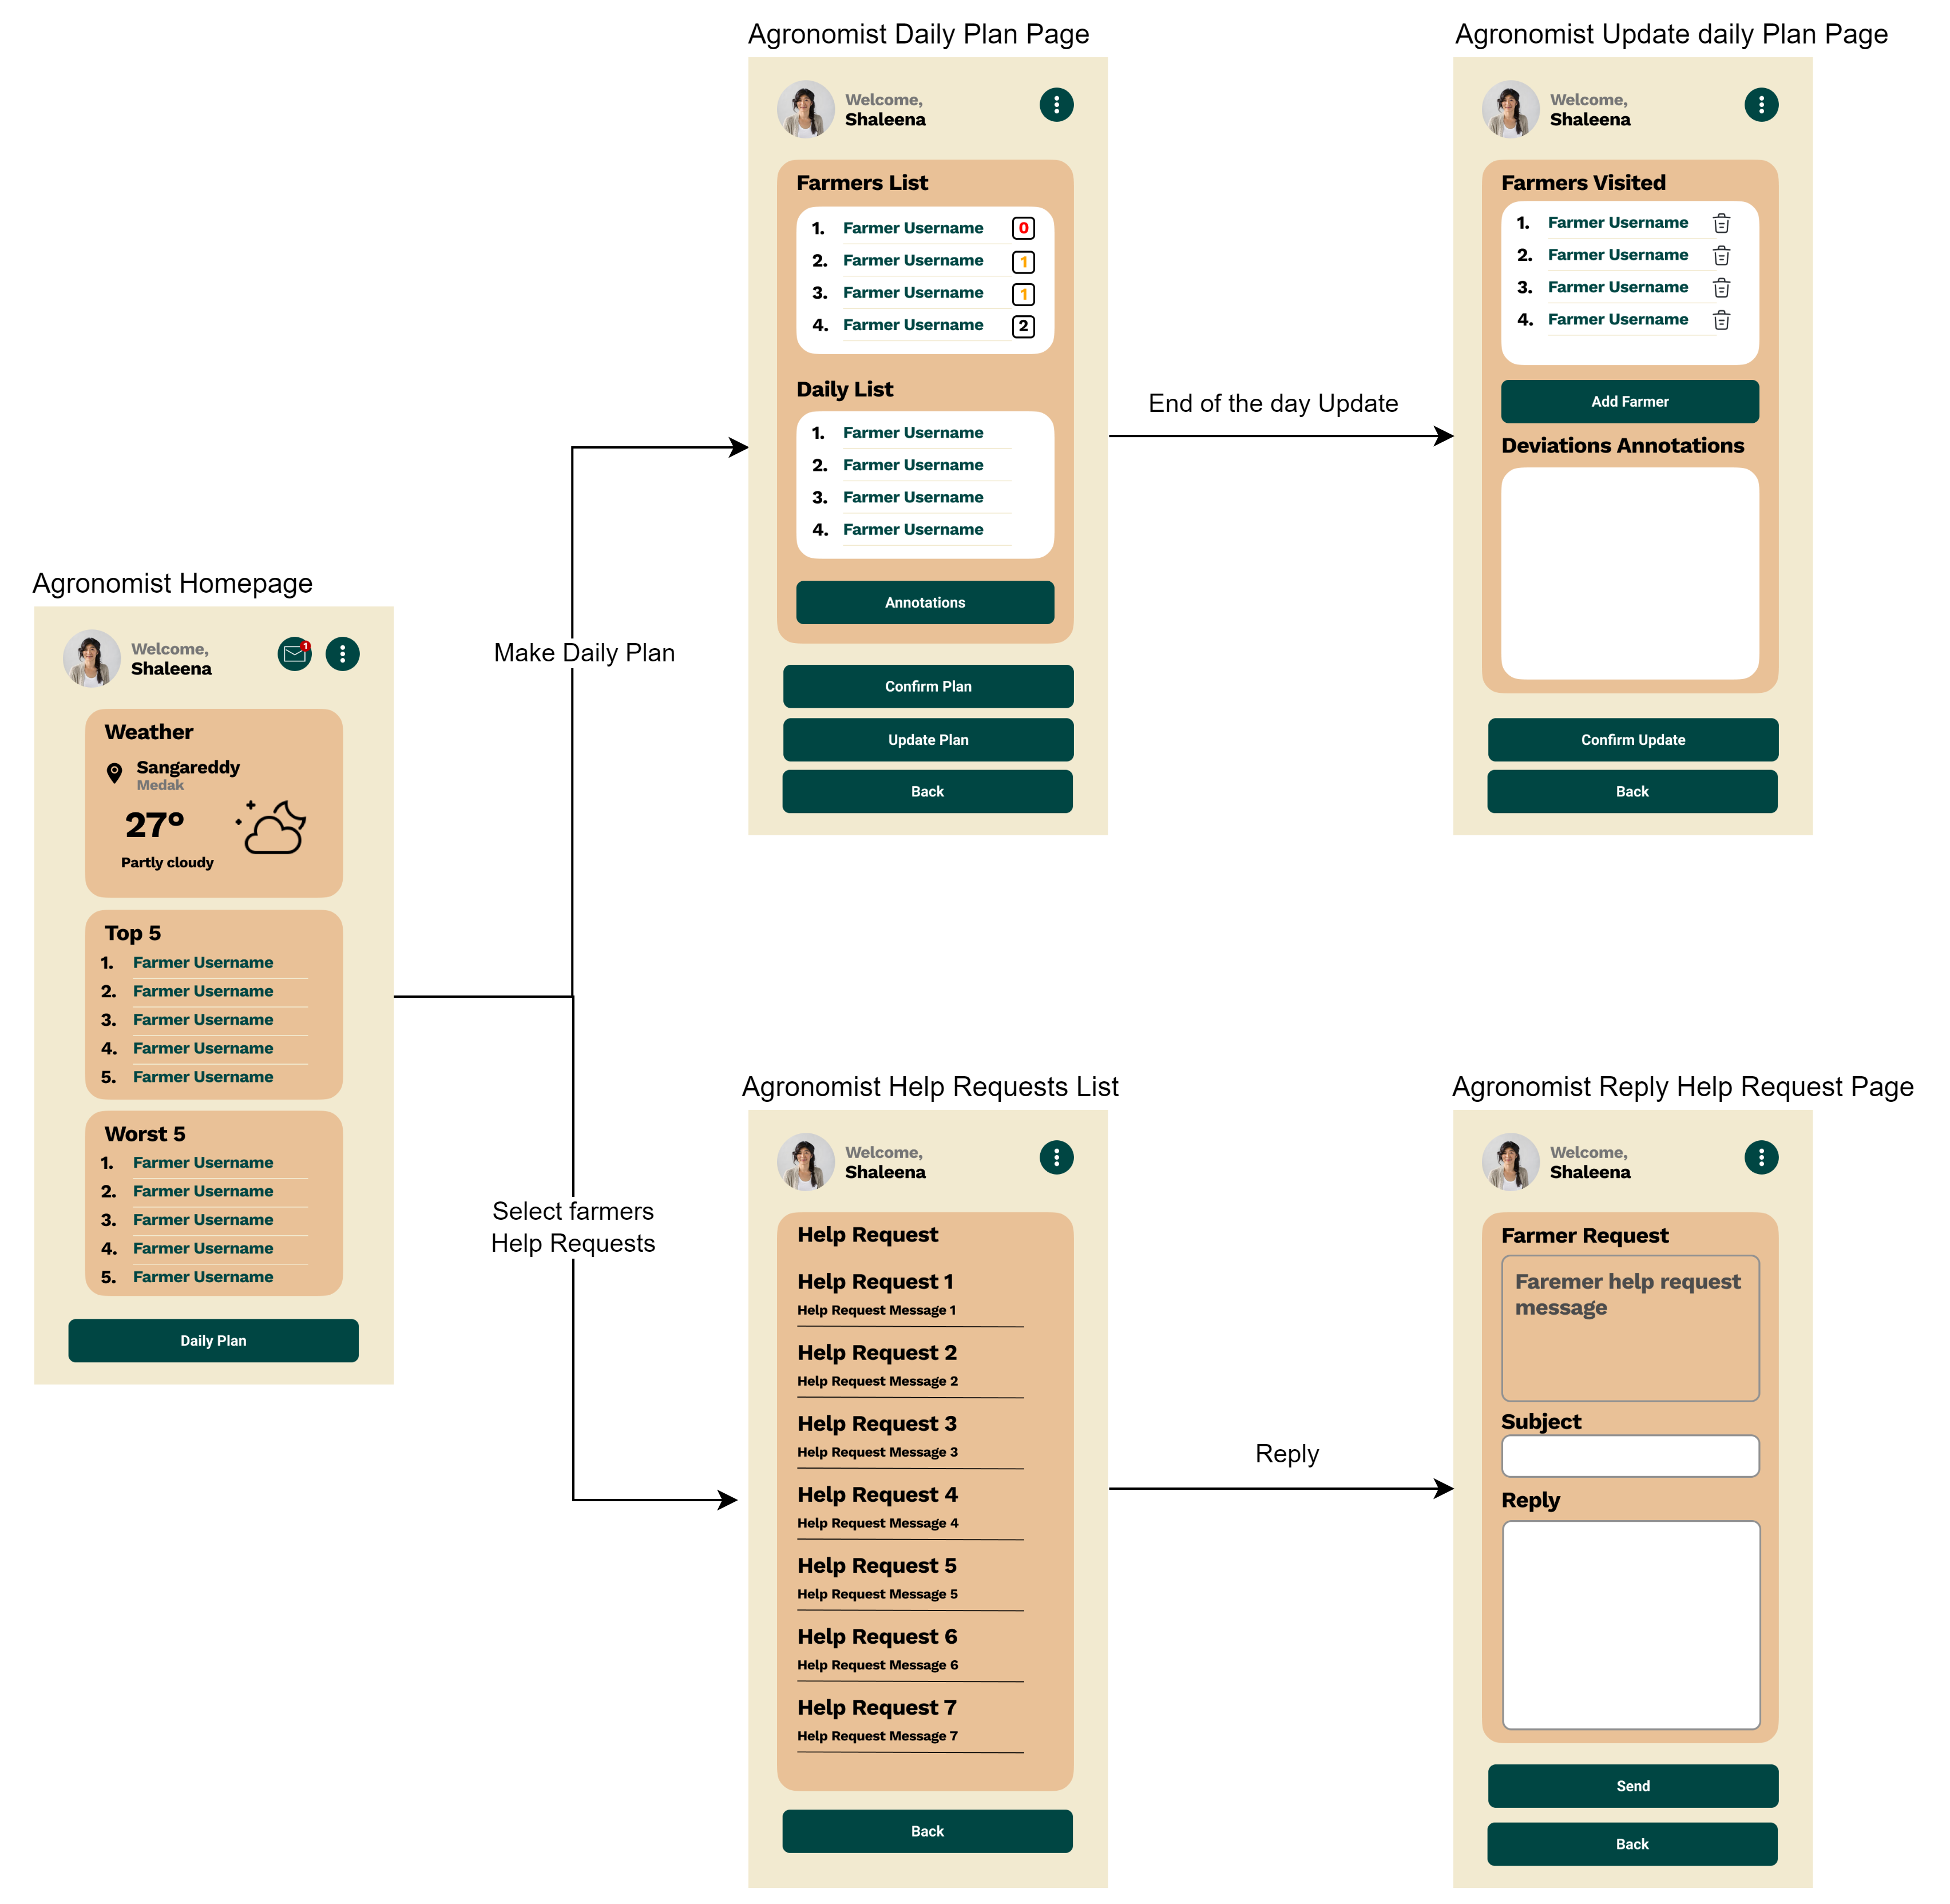
\includegraphics[scale=0.8, center]{assets/MockUp/AgroInteractions.png}
        \caption{Agronomists Interactions}
        \label{fig: agroMockup}
    \end{figure}
\end{center}
\begin{center}
    \begin{figure}[H]
        \vspace{-120px}
        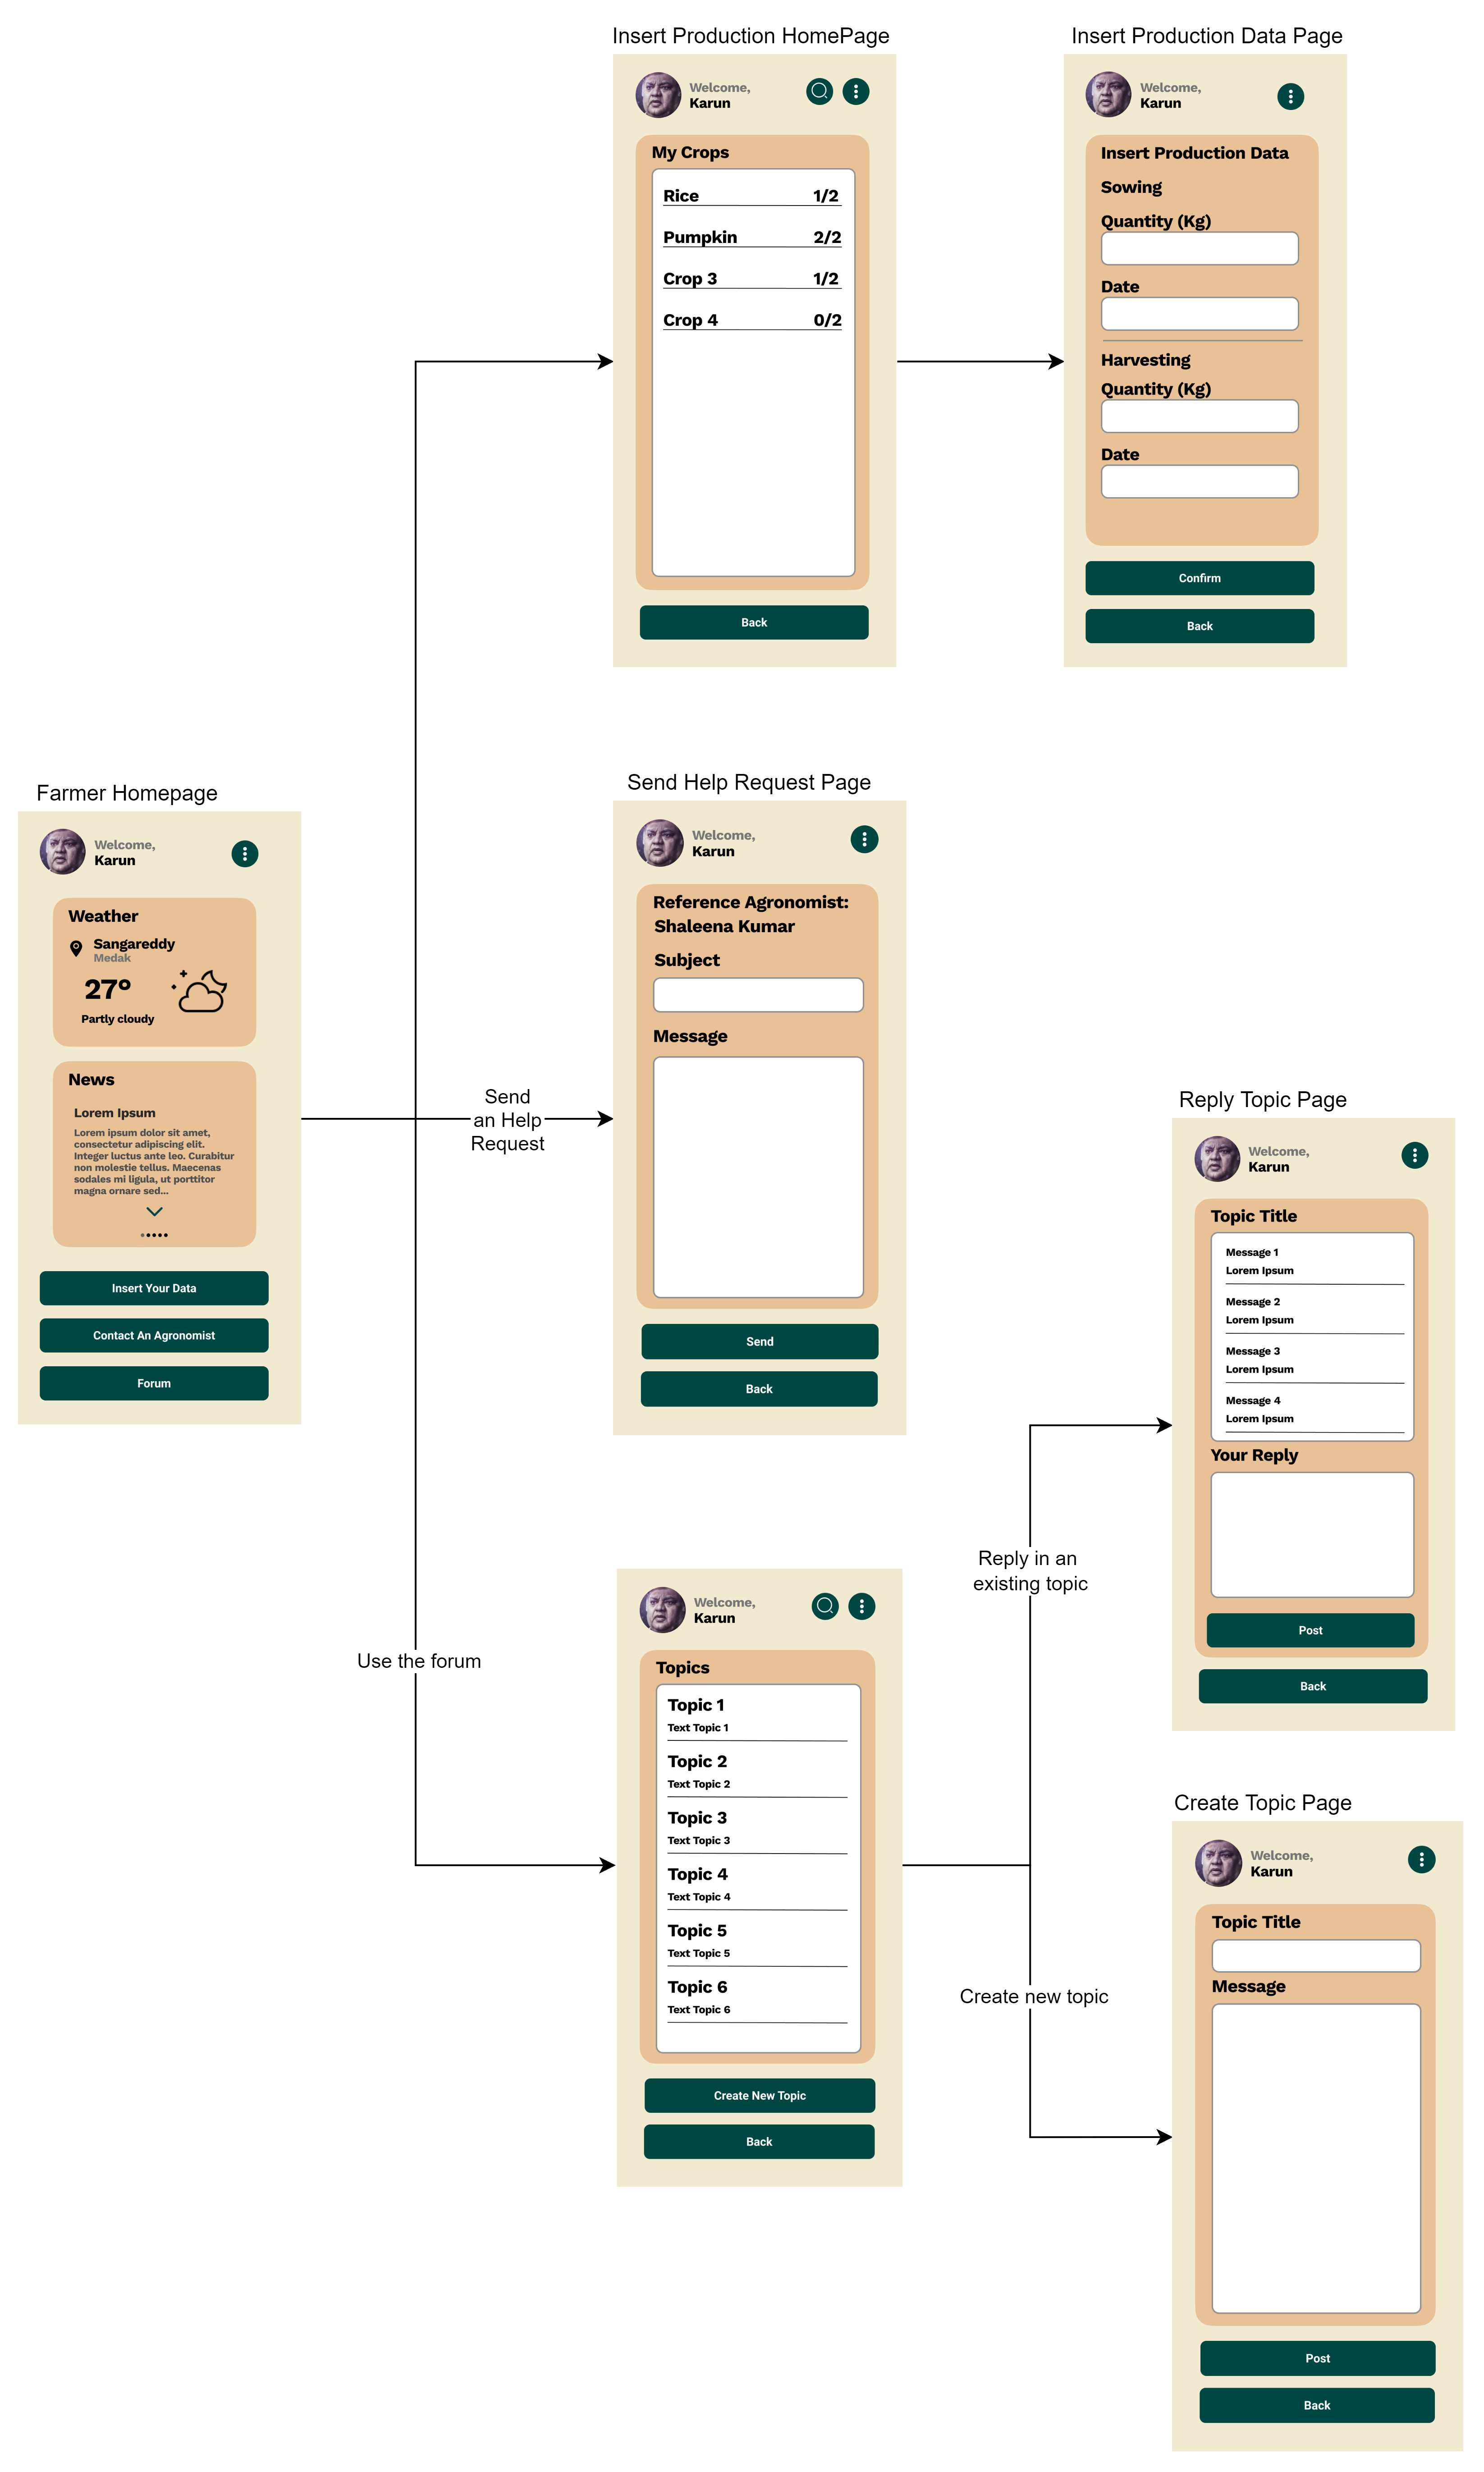
\includegraphics[scale=0.6, center]{assets/MockUp/FarmerInteraction.png}
        \caption{Farmers Interactions}
        \label{fig: farmerInter}
    \end{figure}
\end{center}
\begin{center}
    \begin{figure}[H]
        \vspace{-100px}
        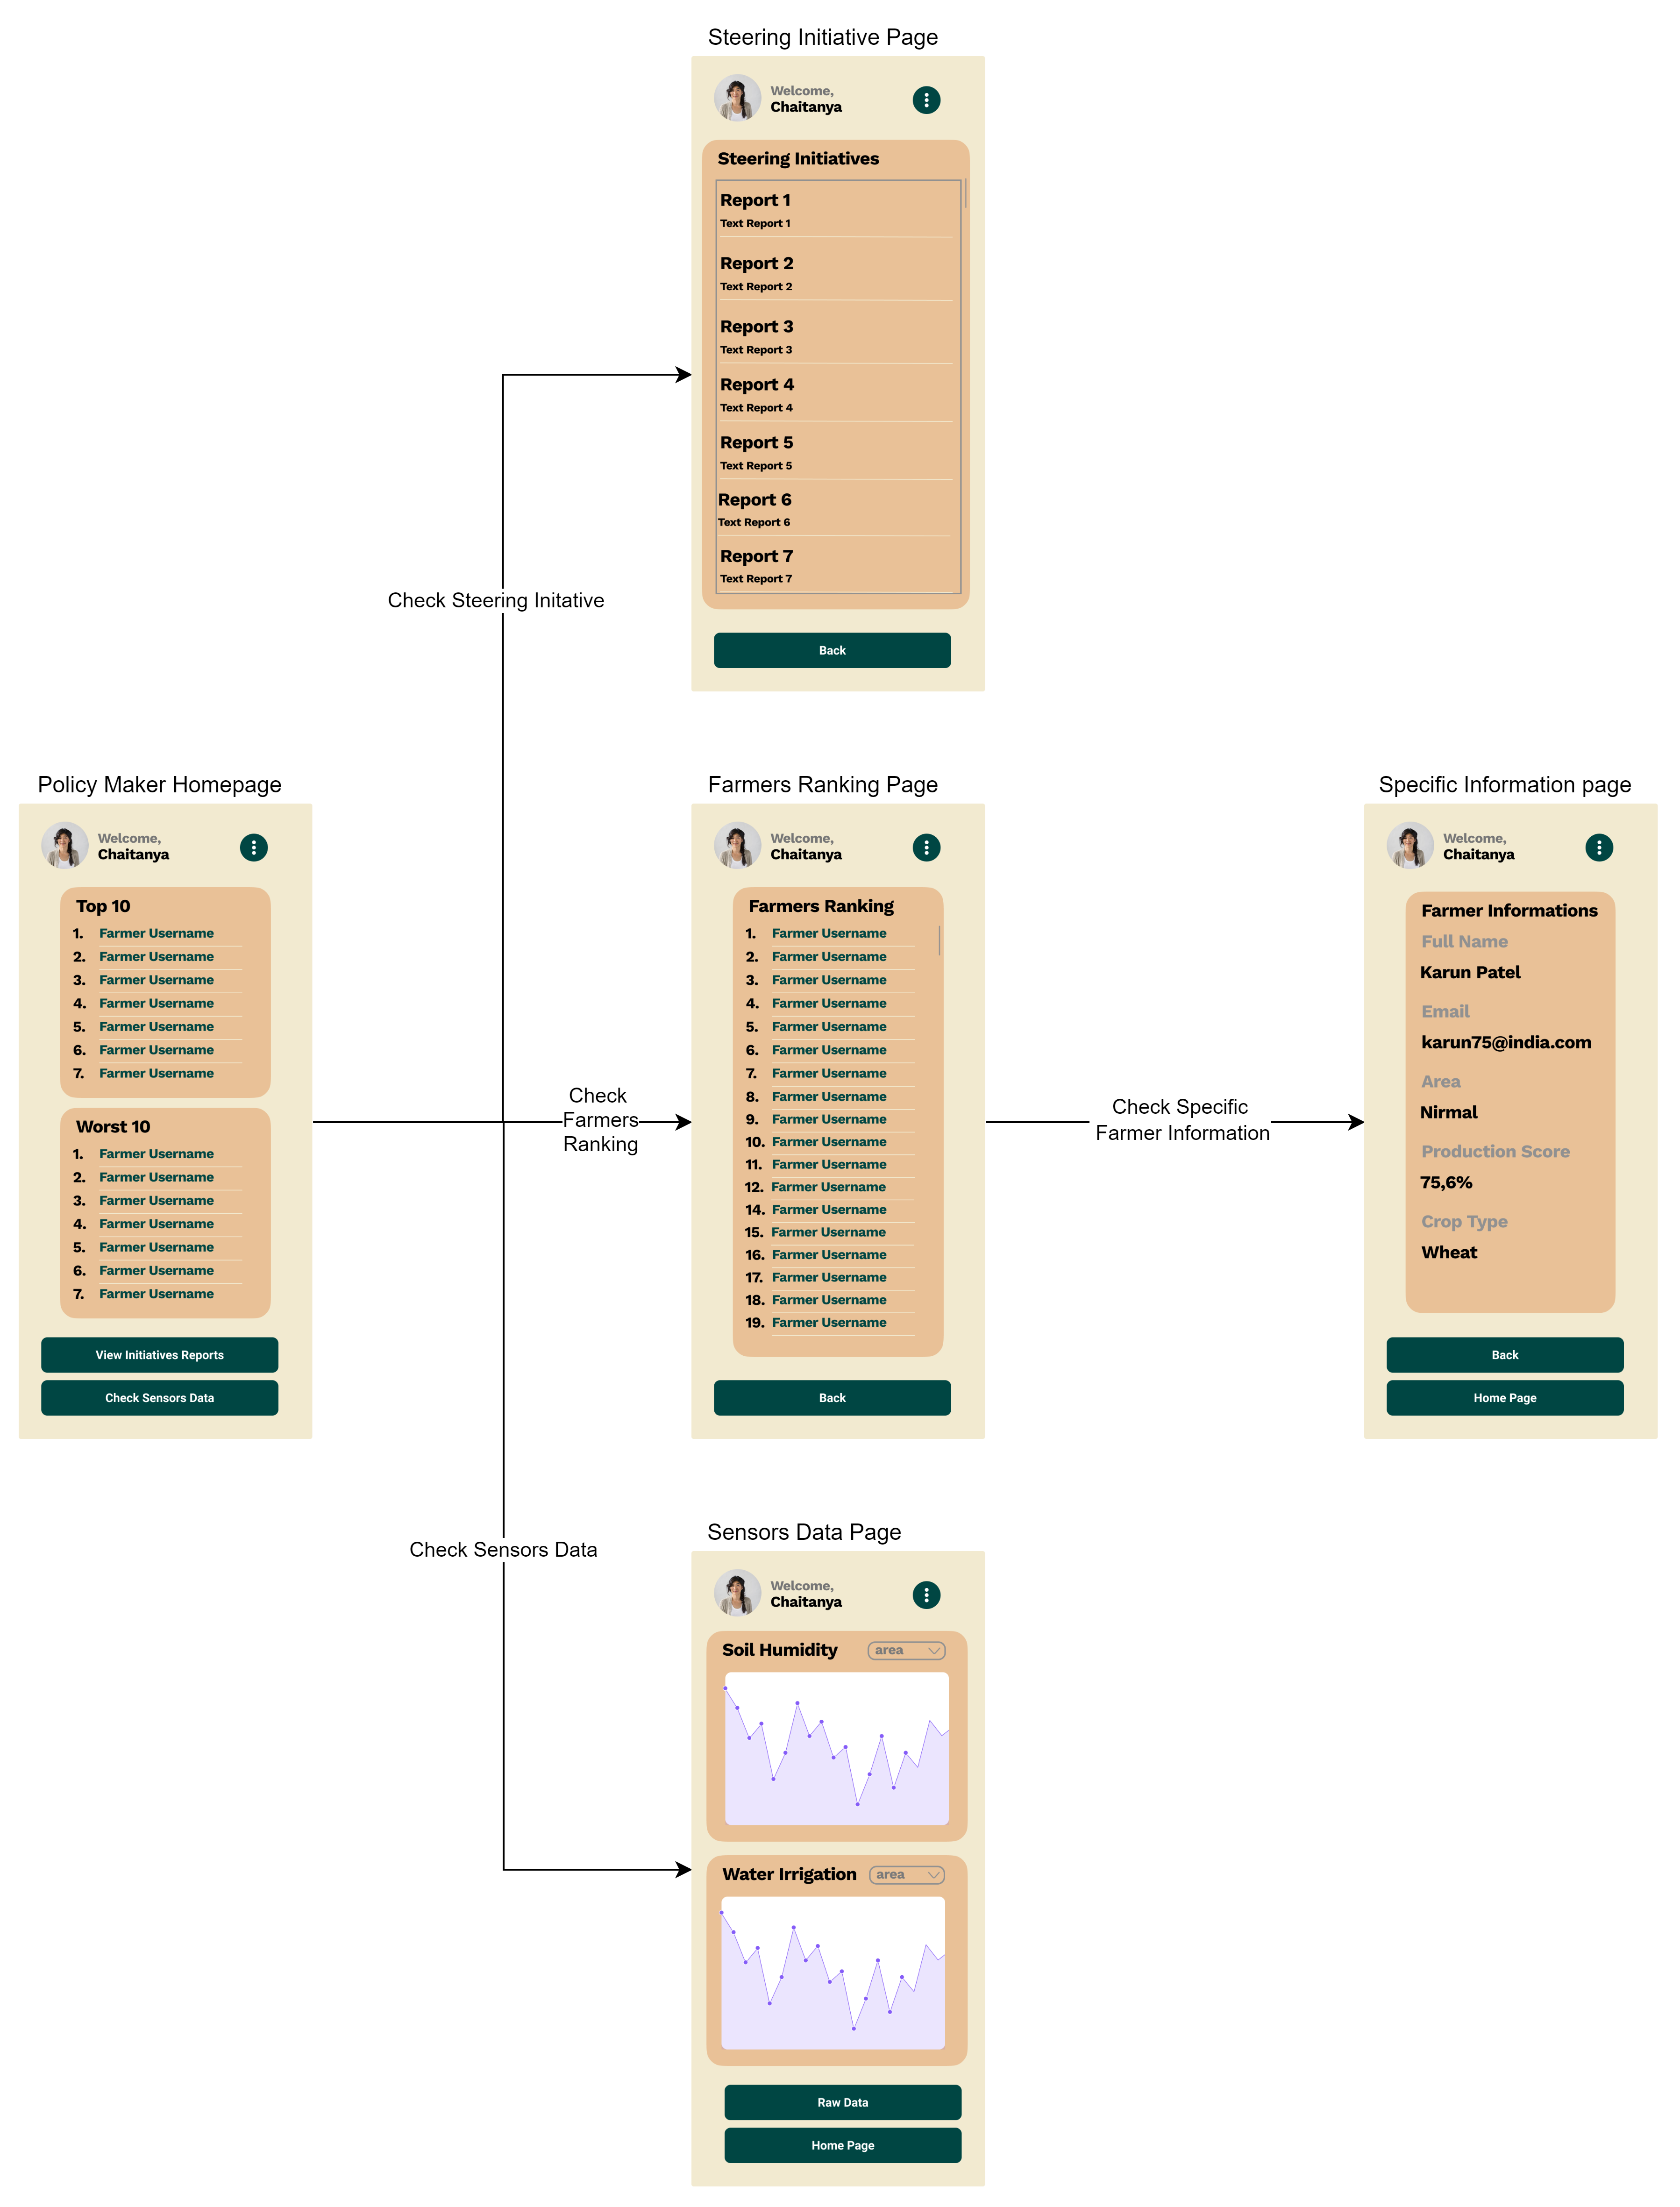
\includegraphics[scale=0.7, center]{assets/MockUp/PMInteractoins.png}
        \caption{Policy Maker Interactions}
        \label{fig: PMInter}
    \end{figure}
\end{center}

\section{Requirements Traceability}

\begin{longtable}{|p{0.47\textwidth}|p{0.45\textwidth}|}
    \hline
    \textbf{Requirements} & \textbf{Components} \\\hline\hline
    \begin{itemize}
        \item[R1)] The system must allow only registered and logged-in users to use the app
        \item[R2)] The system shall allow users to be identified by an email of their choosing
        \item[R3)] The system must suggest to the farmer users the area in which they are during the registration phase if the IT device is equipped with GPS technology. In any case, the final decision will be up to the registering userthe registering user
    \end{itemize}
    & 
    \begin{itemize}
        \item AccountManager
        \item LocationModule
        \item MapServiceManager
    \end{itemize}
    \\\hline

    \begin{itemize}
        \item[R4)] The system must inform the user to try later if they are experimenting connectivity issues
    \end{itemize}
    & 
    \begin{itemize}
        \item AccountManager
    \end{itemize}
    \\\hline

    \begin{itemize}
        \item[R5)] The system must allow Policy Makers to see up-to-date statistic data about water irrigation systems and soil humidty sensors
        \item[R6)] The system must allow Policy Makers to retrieve all agronomists' steering initiative reports uploaded to the database
        \item[R7)] The system must give Policy Makers up-to-date ranking of the best and worst performing farmers  
    \end{itemize}
    & 
    \begin{itemize}
        \item PolicyMakerManager
        \begin{itemize}
            \item WaterIrrigationService
            \item HumiditySensorService
            \item SteeringInitiativeService
            \item RankingService
        \end{itemize}
        \item SteeringInitiativeManager
        \item DataManager
        \item SensorsDataManager
        \item RankingManager
        \item Agronomist
        \begin{itemize}
            \item SteeringInitiativeService
        \end{itemize}
    \end{itemize}
    \\\hline

    \begin{itemize}
        \item[R8)] The system must use a fair and scientific score to rank the Farmers in order to represent the real situation 
    \end{itemize}
    & 
    \begin{itemize}
        \item RankingManager
    \end{itemize}
    \\\hline

    \begin{itemize}
        \item[R9)] The system must let Farmers insert their production information every day 
    \end{itemize}
    &
    \begin{itemize}
        \item FarmerManager
        \begin{itemize}
            \item ProductionService
        \end{itemize}
        \item DataManager
    \end{itemize}
    \\\hline

    \begin{itemize}
        \item[R10)] The system must provide the contact of the agronomist appointed to the area of the farmer requesting professional help
    \end{itemize}
    &
    \begin{itemize}
        \item FarmerManager
        \begin{itemize}
            \item AskRequestService
        \end{itemize}
        \item AgronomistManager
        \item DataManager
        \item HelpRequestManager
    \end{itemize}
    \\\hline

    \begin{itemize}
        \item[R11)] The system must allow every user registered as Farmer to access the forum, to create new discussions and to post replies to already existing ones
    \end{itemize}
    &
    \begin{itemize}
        \item FarmerManager
        \begin{itemize}
            \item ForumService
        \end{itemize}
        \item ForumManager
        \item DataManager
    \end{itemize}
    \\\hline

    \begin{itemize}
        \item[R12)] The system must notify agronomists of unresolved requests of help from Farmers 
    \end{itemize}
    &
    \begin{itemize}
        \item AgronomistManager
        \begin{itemize}
            \item AnswerRequestService
        \end{itemize}
        \item HelpRequestManager
    \end{itemize}
    \\\hline

    \begin{itemize}
        \item[R13)] The system must allow the Agronomists to add a new schedule for the day each day
        \item[R14)] he system must suggest to the Agronomists which farms to visit while planning the Daily Plan based on the number of received visits.
        \item[R15)] The system must suggest to the agronomists only the farms among the ones in their competence area  
        \item[R16)] The system must allow the Agronomists to update their schedule during the day
        \item[R17)] The system must register the already uploaded schedule as definitive at 23:59 of the current day  
    \end{itemize}

    &
    \begin{itemize}
        \item AgronomistManager \begin{itemize}
            \item DailyPlanService
        \end{itemize}
    \end{itemize}
    \\\hline

    \begin{itemize}
        \item[R18)] The system must give Agronomists up-to-date ranking of the best and worst performing farmers in their responsibility area 
    \end{itemize}
    &
    \begin{itemize}
        \item RankingManager 
        \item AgronomistManager
        \begin{itemize}
            \item RankingService
        \end{itemize}
    \end{itemize}
    \\\hline

    \begin{itemize}
        \item[R19)] The system must show weather forecasts relevant to the area concerning the Farmer or the agronomist
    \end{itemize}
    &
    \begin{itemize}
        \item WeatherManager
        \item FarmerManager
        \item AgronomistManager
    \end{itemize}
    \\\hline

    \begin{itemize}
        \item[R20)] The system must present news concerning crop only if relevant to the Farmer's own crop type 
    \end{itemize}
    &
    \begin{itemize}
        \item FarmerManager
        \item NewsManager
    \end{itemize}
    \\\hline
    \begin{itemize}
        \item[R21)] The system must allow Policy Makers to upload their steering initiative reports to the database 
    \end{itemize}
    &
    \begin{itemize}
        \item AgronomistManager
        \begin{itemize}
            \item SteeringInitiativeService
        \end{itemize}
        \item SteeringInitiativeManager
    \end{itemize}\\\hline
\end{longtable}

Here, we present a summary of the table above for a more immediate visualization.
\begin{table}[H]
    \centering
    \begin{tabular}{|l l|}
        \hline
        AccountManager:& AcM\\
        LocationModule:& LM\\
        MapServiceManager:& MSM\\
        PolicyMakerManager:& PMM\\
        AgronomistManager:& AgM\\
        FarmerManager:& FaM\\
        ForumManager:& FoM\\
        DataManager:& DM\\
        HelpRequestManager:& HRM\\
        RankingManager & RM\\
        NewsManager:& NM\\
        WeatherManager:& WM\\
        SensorsDataManager:& SDM\\
        SteeringInitiativeManager& SIM\\\hline
        
    \end{tabular}
    \caption{Components' legend}
\end{table}
\newpage
\setlength\LTleft{-2.5cm}
\begin{longtable}{|c|c|c|c|c|c|c|c|c|c|c|c|c|c|c|}

    \hline
    & \cellcolor{blue!30}AcM & \cellcolor{blue!30}LM & \cellcolor{blue!30}MSM & \cellcolor{blue!30}PMM & \cellcolor{blue!30}AgM & \cellcolor{blue!30}FaM & \cellcolor{blue!30}FoM & \cellcolor{blue!30}DM & \cellcolor{blue!30}HRM & \cellcolor{blue!30}RM & \cellcolor{blue!30}NM & \cellcolor{blue!30}WM & \cellcolor{blue!30}SDM & \cellcolor{blue!30}SIM\\\hline
    \cellcolor{SpringGreen!50}R1 & x & x & x &    &       &       &   &       &  &&    &   &&\\\hline
    \cellcolor{SpringGreen!50}R2 & x & x & x &    &       &       &   &       &  &&    &   &&\\\hline
    \cellcolor{SpringGreen!50}R3 & x & x & x &    &       &       &   &       &  &&    &   &&\\\hline
    \cellcolor{SpringGreen!50}R4 & x &  &  &    &       &       &   &       &  &&    &   &&\\\hline
    \cellcolor{SpringGreen!50}R5 &    & & & x & & && x && & &&x&\\\hline
    \cellcolor{SpringGreen!50}R6 &    & & & x & & && x && & &&x&x\\\hline
    \cellcolor{SpringGreen!50}R7 &    & & & x & & && x && & &&x&\\\hline
    \cellcolor{SpringGreen!50}R8 &    & & & & & && x && & &&&\\\hline
    \cellcolor{SpringGreen!50}R9 &    & & & & & x && x && & &&&\\\hline
    \cellcolor{SpringGreen!50}R10 &    & & & & x & x && x & x & & &&&\\\hline
    \cellcolor{SpringGreen!50}R11 &    & & & & & x & x & x && & &&&\\\hline
    \cellcolor{SpringGreen!50}R12 &    & & & & x &  &&  & x & & &&&\\\hline
    \cellcolor{SpringGreen!50}R13 &    & & & & x &  &&  &  & & &&&\\\hline
    \cellcolor{SpringGreen!50}R14 &    & & & & x &  &&  &  & & &&&\\\hline
    \cellcolor{SpringGreen!50}R15 &    & & & & x &  &&  &  & & &&&\\\hline
    \cellcolor{SpringGreen!50}R16 &    & & & & x &  &&  &  & & &&&\\\hline
    \cellcolor{SpringGreen!50}R17 &    & & & & x &  &&  &  & & &&&\\\hline
    \cellcolor{SpringGreen!50}R18 &    & & & & x &  &&  &  & x & &&&\\\hline
    \cellcolor{SpringGreen!50}R19 &    & & & & x & x &&  &  & & & x &&\\\hline
    \cellcolor{SpringGreen!50}R20 &    & & & & & x &&  &  & & x &&&\\\hline
    \cellcolor{SpringGreen!50}R21 & &&&& x &&&x &&&&&&x\\\hline
    \caption{Component and requirement mapping}\\
\end{longtable}

\section{Implementation, Integration and Test Plan}
\subsection{Implementation Plan}
Multiple components will be implemented at the same time, in order to parallelize the development when possible. The general plan is to follow a bottom-up approach, so that core and basic functionalities with very few dependencies can be tested as soon as their incapsulating component is done. By doing so, the application will be built up with solid and tested foundations that will ease the further testing of bigger and complex components. In any case, unit testing will be performed on each component on the go, in order to find flaws out in advance. This will positevely impact the necessary actions to fix the faults since they will be done in an earlier stage.

The implementation's order of the component will be as follow:
\begin{enumerate}
    \item DataManager, MapServiceManager, WeatherManager, SensorDataManager, NewsManager
    \item RankingManager, SteeringInitiativeManager, HelpRequestsManager, ForumManager, LocationModule
    \item PolicyMakerManager, AgronomistManager, FarmerManager, AccountManager
\end{enumerate}
Each group is composed by independent modules so they can be easily developed in parallel.
Furthermore, it is expected that external services (e.g. GoogleMapsAPI, OpenWeatherAPI, WaterIrrigationAPI, HumiditySensorsAPI, NewsAPI and DBMS Service) work properly since they're not a responsibility of the DREAM app.

The \emph{DataManager} component should be implemented first since all the remaining components of the application server depend directly or indirectly on it for handling the communication with the database to store and retrieve data. \emph{MapServiceManager}, \emph{WeatherManager}, \emph{SensorDataManager} and \emph{NewsManager} components are independent from all the other ones because the former just communicates with the external services, by modifying the API's information so that it can be comprehensible by the Application server, and adapting the requests to the API's protocol.

The second group depends on the first one but at the same time incapsulates building blocks for the third one.  \emph{RankingManager}, \emph{SteeringInitiativeManager}, \emph{HelpRequestsManager} and \emph{ForumManager} directly exploit the \emph{DataManager} module to retrieve information, store data or carry out consistency and security checks. Moreover, \emph{LocationModule} also use the \emph{MapServiceManager} to access the map service that ease the registration to the farmers in localizing their farm. 

Finally, \emph{PolicyMakerManager}, \emph{AgronomistManager}, \emph{FarmerManager} and \emph{AccountManager} are the component that mostly depend on all the lower level ones, as can be seen in figure \ref{fig: application_server_component_view}.
\subsection{Integration Strategy}
Considering both the overall system's architecture and the implementation
plan, the chosen integration strategy is the bottom-up approach. System
integration begins with the integration of the lowest level modules and uses
test drivers to drive and pass appropriate data to the lower-level modules. As
and when the code for the other module gets ready, these drivers are replaced
with the actual module.

This approach allows to start the integration and testing without necessarily
waiting for the completion of the development and the unit testing of each
system's component. Being the low-level modules and their combined functions
often invoked by other modules, it is more useful to test them first so that
meaningful effective integration of other modules can be done. Moreover,
starting at the bottom of the hierarchy means that the critical modules are built
and tested first and therefore any errors in these modules are identified early in
the process.

Each integration in the same level (defined by the groups of the previous
section) is independent and there is no specific order in which to complete them.
In this way, the integration process and its testing are more flexible.

\subsubsection{Integration and Testing}
In this section it is defined the order of the integration between components. Test drivers will be used to simulate higher components not yet implemented.
As already said, bottom-up approach is going to be followed in implementing the components. So firstly, \emph{DataManager} (fig. \ref{fig: integration_DataManager}), \emph{MapServiceManager} and \emph{WeatherManager} (fig. \ref{fig: integration_MapServiceManager_WeatherManager}), \emph{SensorDataManager} and \emph{NewsManager} (fig. \ref{fig: integration_SensorDataManager_NewsManager}) are implemented using drivers for higher-up components yet to be built.

\begin{figure}[H]
    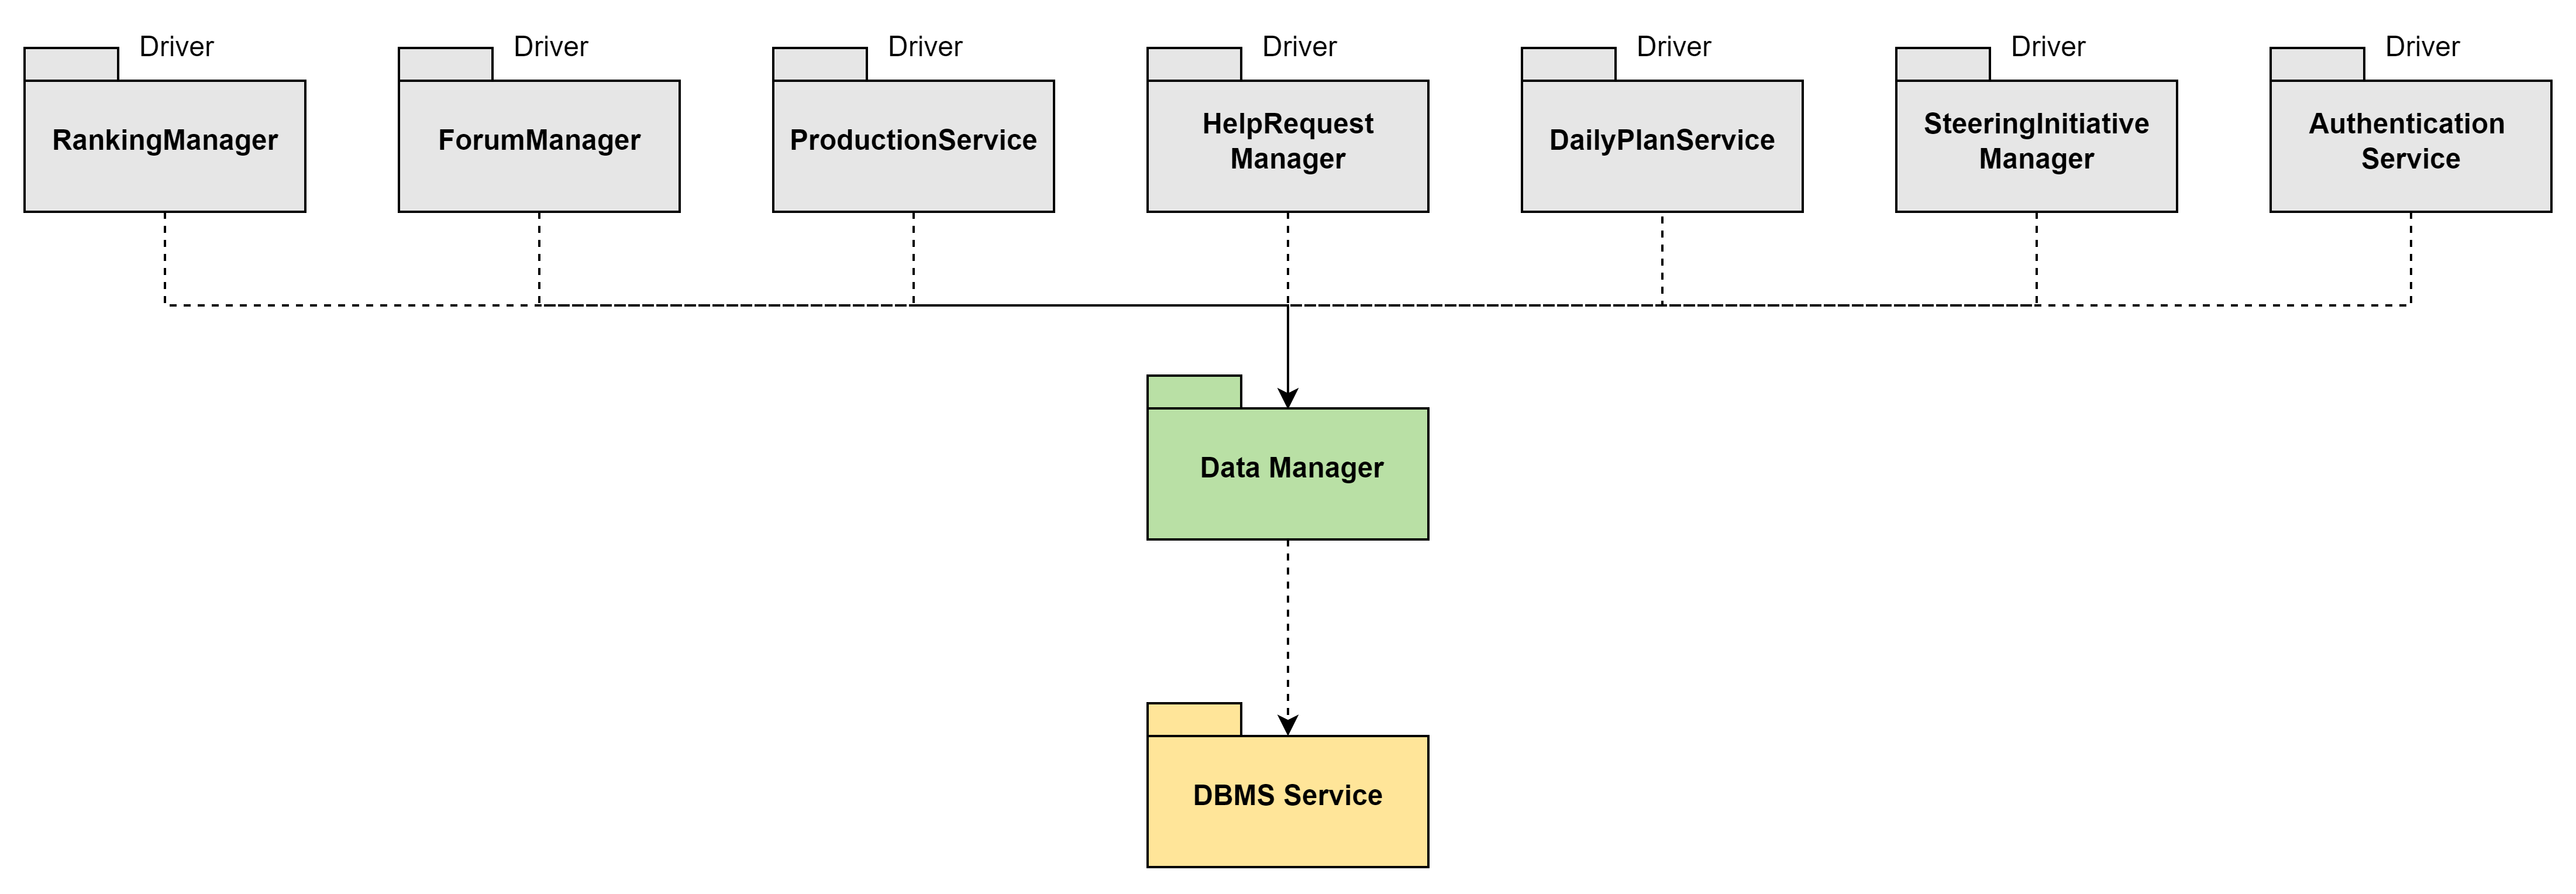
\includegraphics[scale=0.5, center]{assets/Test/generalTest.png}
    \caption{Integration of DataManager component}
    \label{fig: integration_DataManager}
\end{figure}

\begin{figure}[H]
    \centering
    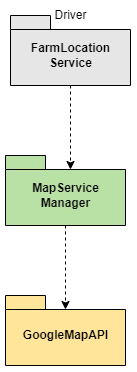
\includegraphics[scale=0.56]{assets/Test/farmLocationTest.png} 
    \caption{Integration of MapServiceManager component}%
    \label{fig: integration_MapServiceManager_WeatherManager}%
\end{figure}

\begin{figure}[H]
    \centering
    \subfloat[\centering SensorDataManager]{{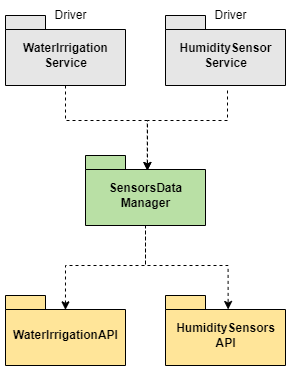
\includegraphics[scale=0.5]{assets/Test/sensorsTest.png}}}%
    \qquad\qquad
    \subfloat[\centering NewsManager]{{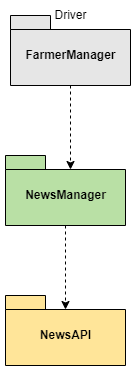
\includegraphics[scale=0.5]{assets/Test/newsTest.png}}}%
    \caption{Integration of SensorDataManager and NewsManager components}%
    \label{fig: integration_SensorDataManager_NewsManager}%
\end{figure}

After the first group implementation and testing, it's time for the implementation of the middle tier: \emph{RankingManager} and \emph{HelpRequestManager} (fig. \ref{fig: integration_RankingManager_HelpRequestManager}) and \emph{ForumManager}(fig. \ref{fig: integration_ForumManager_LocationModule}).
\begin{figure}[H]
    \centering
    \subfloat[\centering RankingManager]{{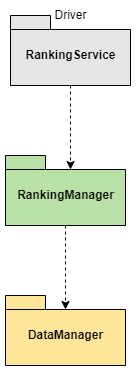
\includegraphics[scale=0.5]{assets/Test/rankingTest.png}}}%
    \qquad\qquad
    \subfloat[\centering HelpRequestManager]{{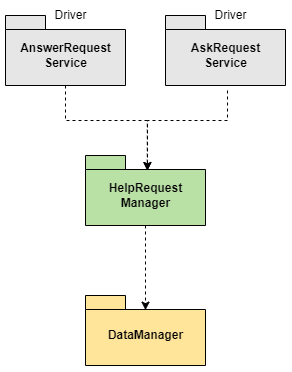
\includegraphics[scale=0.5]{assets/Test/helpTest.png}}}%
    \caption{Integration of RankingManager and HelpRequestManager components}%
    \label{fig: integration_RankingManager_HelpRequestManager}%
\end{figure}
\begin{figure}[H]
    \centering
    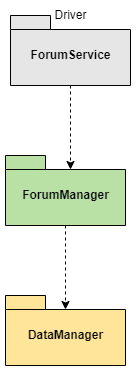
\includegraphics[scale=0.5]{assets/Test/forumTest.png}%
    \caption{Integration of ForumManager component}%
    \label{fig: integration_ForumManager_LocationModule}%
\end{figure}

Finally, the last group, composed by the components with most dependencies, doesn't require drivers to do integration testing, they just rely on the already built modules underneath. The integration testing to carry out for \emph{PolicyMakerManager}, \emph{AgronomistManager}, \emph{FarmerManager} and \emph{AccountManager} are presented in the following figure respectively: \ref{fig: integration_PolicyMakerManager}, \ref{fig: integration_AgronomistManager}, \ref{fig: integration_FarmerManager}, \ref{fig: integration_AccountManager}.

\begin{figure}[H]
    \centering
    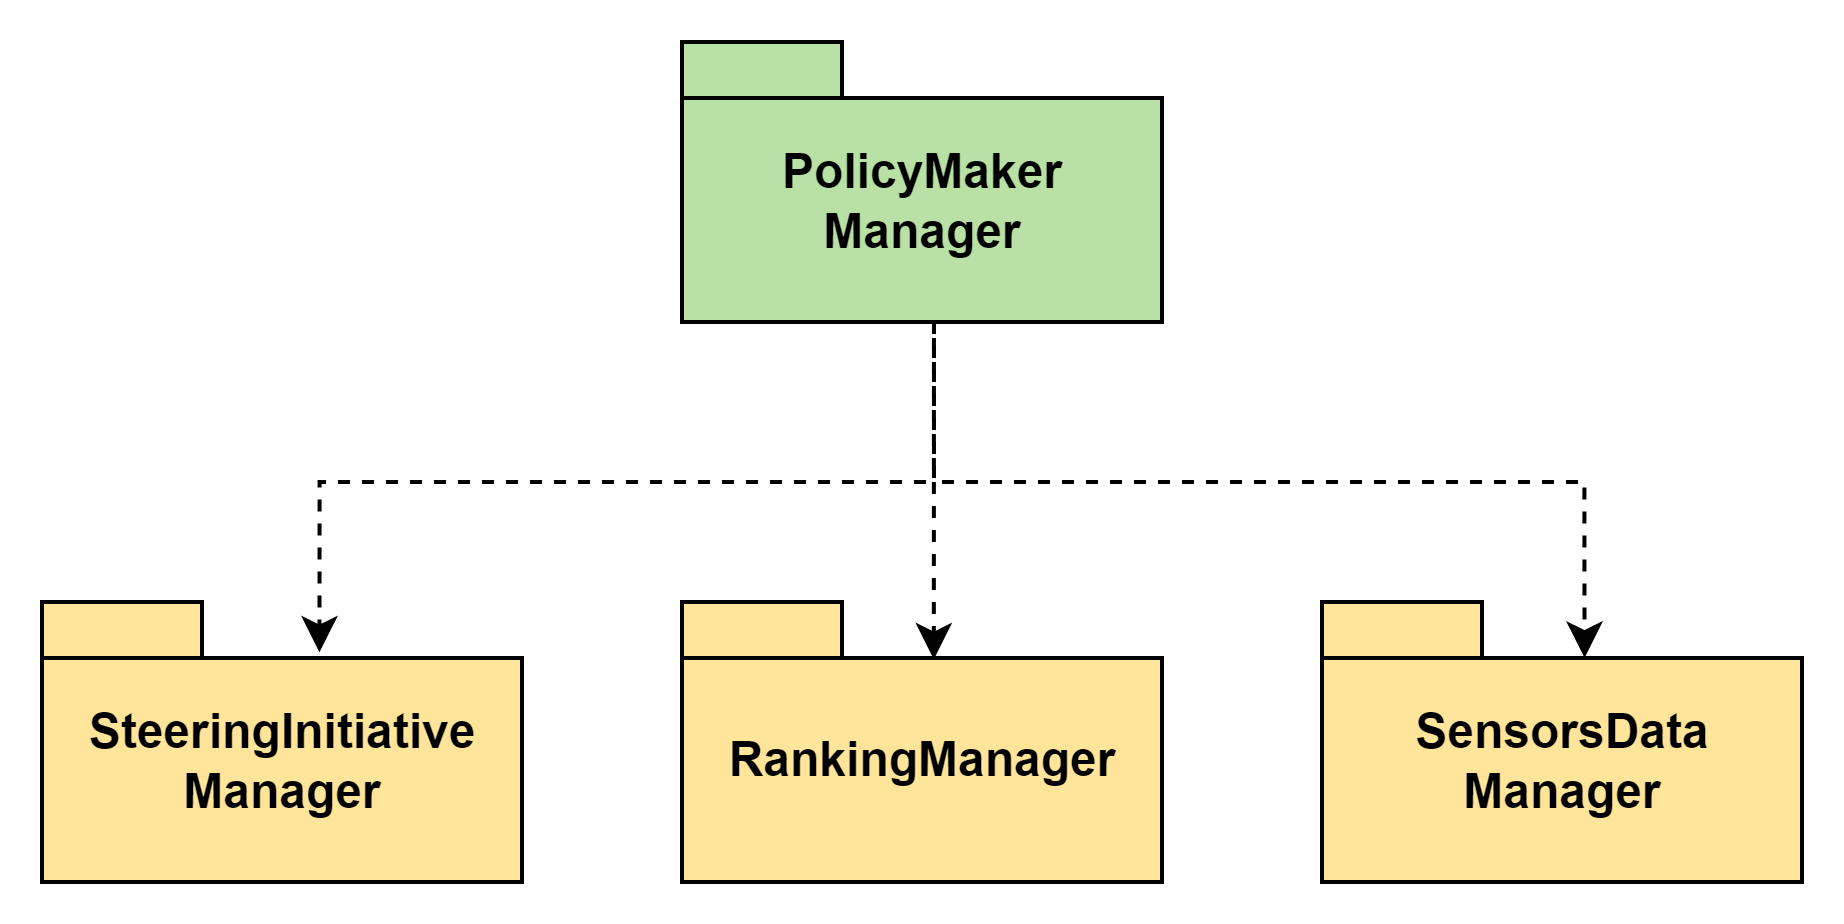
\includegraphics[scale=0.5, center]{assets/Test/pmTest.png}
    \caption{Integration of PolicyMakerManager components}
    \label{fig: integration_PolicyMakerManager}
\end{figure}
\begin{figure}[H]
    \centering
    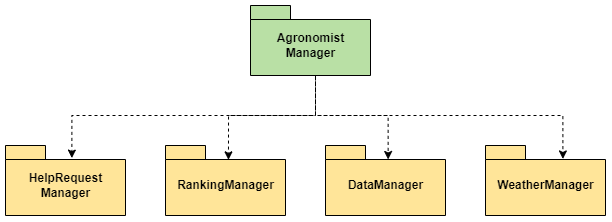
\includegraphics[scale=0.5, center]{assets/Test/agroTest.png}
    \caption{Integration of AgronomistManager components}
    \label{fig: integration_AgronomistManager}
\end{figure}
\begin{figure}[H]
    \centering
    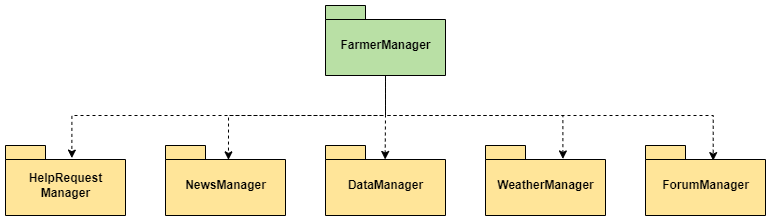
\includegraphics[scale=0.5, center]{assets/Test/farmerTest.png}
    \caption{Integration of FarmerManager components}
    \label{fig: integration_FarmerManager}
\end{figure}
\begin{figure}[H]
    \centering
    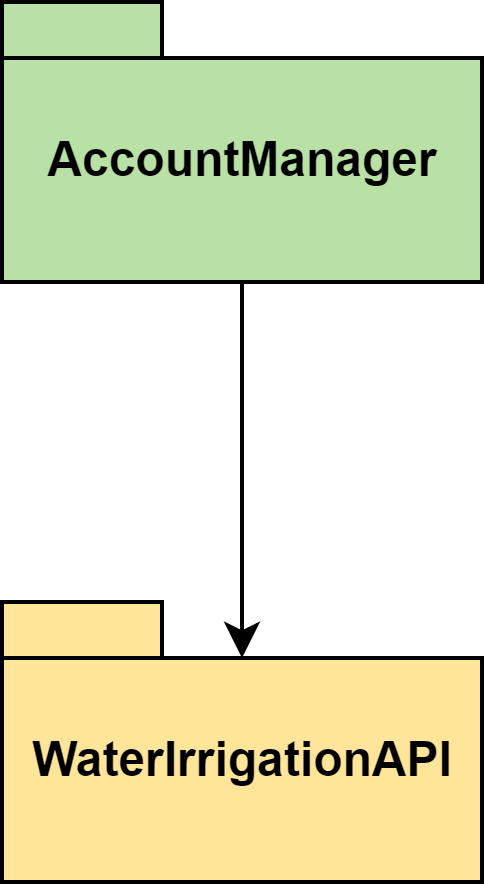
\includegraphics[scale=0.5, center]{assets/Test/accountTest.png}
    \caption{Integration of AccountManager components}
    \label{fig: integration_AccountManager}
\end{figure}

\subsection{System testing}
Once the whole application has been implemented and tested, the application server can be integrated in the whole distributed system. This brings new testing phases to carry out: stress and load testing. The purpose of these is to achieve data regarding availability. Load testing is especially important because of the high expect demand of users that will use the system. On the same note, performance testing would allow us to know the response time of the most frequent operations and requests such as retrieving sensors' data, ranking visualization, posting on the forum, weather forecast and news visualization, sending an help request and replying to one, retrieving of agronomists' reports, etc. Performance testing is a key aspect to fulfilling the RASD non-functional requirement of needing a response time of 0.5s. Moreover, the testing should consider important algorithms such as the retrieval of data from the database (queries and insertions) or response time from external APIs.

\newpage
\section{Effort Spent}
    \begin{tabular}{|c||c|c|c|c|c|}
        \hline
        Student & Time for S.1 & S.2 & S.3 & S.4 & S.5\\ \hline
        Ottavia Belotti & 1h & 7h & 2h & 4h & 7h \\
        Alessio Braccini & 2h & 8h & 8h & 1h  & 2h \\
        Riccardo Izzo & 2h & 15h & 2h & 1h  & 1h \\
        \hline
    \end{tabular}


\section{References}


\begin{thebibliography}{9}
    \bibitem{mvc}
    MDN Web Docs Glossary: Definitions of Web-related terms -> MVC
    \url{https://developer.mozilla.org/en-US/docs/Glossary/MVC}

    \bibitem{rainfallsData}
    Rainfall state in Telangana: \url{https://www.tsdps.telangana.gov.in/aws.jsp}
    
\end{thebibliography}

\end{document}